\documentclass[11pt]{article}
\usepackage{graphicx}
\usepackage{epsfig}
\usepackage{url}
\usepackage[english]{babel}
\usepackage{vmargin}
\usepackage{times}
\usepackage{amssymb}
\usepackage[fleqn]{amsmath}
\usepackage{cite}
\usepackage{titling}
\usepackage{color}
\usepackage{xspace}
\usepackage{listings}
\usepackage{upquote}
\usepackage[hidelinks]{hyperref}
\usepackage{wrapfig}
\setpapersize{USletter}
\usepackage{textpos}
\usepackage{enumitem}
\usepackage{tikz}
\usepackage{tikz-qtree}
\usepackage{rotating}
\usepackage{float}
\usepackage{geometry}
\usepackage{lscape}
\usepackage{graphicx} 
\usetikzlibrary{external,automata,trees,positioning,shadows,arrows,shapes.geometric}

\setlength{\textheight}{220mm}
\setlength{\textwidth}{160mm}
\evensidemargin=0.5in
\oddsidemargin=1.1in
\topmargin=0.45in
\usepackage[compact,noindentafter]{titlesec}
\titlespacing{\section}{0pt}{*2.4}{*1.8}
\titlespacing{\subsection}{0pt}{*2.0}{*1.6}
\titlespacing{\subsubsection}{0pt}{*1.6}{*1.2}
\renewcommand{\baselinestretch}{1.25}

\newcommand{\fulltitle}{\textbf{Malware Analysis for Proactive Detection and Prevention\xspace}}
\title{\fulltitle}
\date{}
%\author\textit{Tejas Khairnar (1207690220, Group Leader) \\Sujay Vaishampayan (1209248166, Deputy Group Leader)\\  Zhibo Sun(1207644187)\\Harshil Maskai (1209174092)\\ Aloma Lopes (1209273126)\\ Chaitanya Palaka (1209261868)\\ Varun Chandrasekar (1209248010) \\ Kunal Bansal (1211213169) \\ Raj Dalvi (1209232176) \\ Vimal Vadivelu (1209203043)\\ \\

\begin{document}
	\begingroup
		\fontsize{20pt}{20pt}\selectfont
		\begin{center}
			Arizona State University \\~\\
			CSE 543 Information Assurance and Security
		\end{center}
	\endgroup
	{\let\newpage\relax\maketitle}
	\begingroup
	\fontsize{15pt}{15pt}\selectfont
	\begin{center}
		\textit{Tejas Khairnar (1207690220, Group Leader) \\Sujay Vaishampayan (1209248166, Deputy Group Leader)\\  Zhibo Sun(1207644187)\\Harshil Maskai (1209174092)\\ Aloma Lopes (1209273126)\\ Chaitanya Palaka (1209261868)\\ Varun Chandrasekar (1209248010) \\ Kunal Bansal (1211213169) \\ Raj Dalvi (1209232176) \\ Vimal Vadivelu (1209203043)}
	\end{center}
	\endgroup
	\begin{abstract}
		\textbf{\textit{There are a multitude of potentially malicious samples out there in the wild. The signatures for these malwares are mainly created manually. This creates a semantic gap while detecting known pieces of malware and unknown pieces of malwares. This survey article provides an overview of various techniques used to perform malware analysis, detect and prevent them. It also covers various strategies to detect these malwares pro-actively and be one step ahead of the attackers.}}
	\end{abstract}
		\begingroup
		\fontsize{10pt}{10pt}\selectfont
			\begin{center}
				Spring 2017, Group \#2 \\~\\
				March 27, 2017
			\end{center}
		\endgroup


	\newpage
	\tableofcontents
	\newpage
	% This puts the word "Page" right justified above everything else.
	\addtocontents{toc}{~\hfill Page\par}
	\listoftables
	\newpage
	\listoffigures
	\newpage
	\section{Introduction}
	\subsection{Background and Motivation}
	In today’s world connected by the Internet, cyber security has become a major concern. In order
to be secure, software as well as hardware industries around the world are working proactively to
secure their software and stay secured. One of the major threats to these industries arises due to
malware which can be defined as a small piece of software that is intended to damage or disable
computers and computer systems. Hence our research survey is focused on studying techniques
to proactively detect and defend against these malwares.\\ Stuxnet~\cite{creators2013kill, stuxnet} considered to be the most sophisticated piece of malware ever detected was used in operations against Iran in 2010. Stuxnet was so sophisticated and complicated that it was believed that this malware could be developed and deployed only with fundings which rivals that of the military of a nation. Stuxnet is unique in its own nature because unlike other Viruses or Worms it targets systems that are traditionally not connected to the internal network, which can also be termed as isolated machines. It infected Windows machines through USB keys and then propagated across the network scanning for Siemens Step7 software on computers controlling Programmable Logic Controllers (PLC). This helped the malware to use the information it gathered to take control of other systems and crash them upon infection. Stuxnet even provided fake feedback to the main controllers outside the network, leading the other systems to believe that the infected computer is functioning normally. All these efforts were part of a Cyber War waged against the Iranian Nuclear Program in order to slow it down. \\
The above example inspires us with the need to be aware about cyber security and how it might affect our cyber world. Many organizations like Kaspersky labs, CrowdStrike are constantly developing expertise to detect these kind of malwares and Trojans spreading around the world. Therefore, we found this area,'Malware Analysis for Proactive Detection and Prevention', very intriguing and considered it to be the center of our research survey.
	\subsection{Goals and scope}
	Our goal for this research survey is to explore and scrutinize various techniques to perform Malware Analysis and understand its application in the real world for proactive defense. We also intend to study various techniques used in order to develop automated malware analysis tools. This will let us compare these techniques and think about coming up with a new strategy by mix and matching them. To explain proactive defense, we need to study literature not just by the research \& academia industry but also from the corporate community. In our scope, to achieve this we also study white papers from certain renowned security companies in the wild. 
	The scope of our research survey encompasses the following areas:
	\begin{itemize}[noitemsep]
		\item{Various Tools and techniques to perform Malware Analysis}
		\item{Techniques to prevent IT Network from Malwares} 
		\item{Techniques to perform Malware Analysis on Android Systems}
		\item{Techniques for proactive detection and prevention of Malwares}
	\end{itemize}
	In order to achieve our goal, each member of our group has reviewed about at least four popular techniques or tools in the research category that was assigned to them. Each paper was carefully selected after considering the most rampant malwares that currently exist in the world and some of the best techniques that are used to defend systems against such malwares.

\section{Overview}
This section talks about specific tasks completed by each group member till date.
\subsection{Tejas Khairnar (1207690220, Group Leader)}
I, as the Group Leader, am organizing weekly meetings with the whole team. My duties include keeping a check on work done by every group member.
I am also helping everyone with finding good papers in the area of 'Malware Analysis Techniques'. Apart from that I have also been reading the research paper "Toward automated dynamic malware analysis using cwsandbox"~\cite{willems2007toward}. \\
I summarized the paper ~\cite{willems2007toward} and studied a research survey on automated malware analysis techniques ~\cite{egele2012survey}. Besides this I worked on the compilation of the whole report in \LaTeX as per project guideline requirements. I made sure that the format of the report is crisp and according to the submission guidelines. I majorly worked on the results section and the story behind the whole paper. 

\subsection{Sujay Vaishampayan (1209248166, Deputy Group Leader)}
I, as the Deputy Group Leader, help the Group Leader in organizing weekly meetings and making sure that deadlines are met. I also helped the members of our group by guiding them on how to write their part of the report. As far as my research category goes, I have studied all the tools which help to perform Malware Analysis using Hardware Virtualization Extensions. This included a detailed description of the tools developed over the years starting from Ether~\cite{dinaburg2008ether} to the latest one which is DRAKVUF~\cite{lengyel2014scalability}. I covered different ways to leverage hardware virtualization to perform malware analysis ranging from tools external to the guest operating system such as V2E~\cite{yan2012v2e} and SPIDER~\cite{dongyan2013spider} to techniques which involve observing the guest operating system from within itself such as Process Implanting~\cite{jiang2011procimplant}. I have extensively covered almost every popular tool in this category of malware analysis and have gained immense knowledge from the same.


\subsection{Zhibo Sun(1207644187)}
	In order to have a new point of view to proactively predict and prevent malwares, we are not only considering the analysis of the malware, but also the threat and malware intelligence. In order to have knowledge in this section, the paper I read was ”Needles in a Haystack: Mining Information from Public Dynamic Analysis Sandboxes for Malware Intelligence~\cite{graziano2015needles} ” that was published in 2015 USENIX SECURITY.
	This paper proposed a novel methodology to automatically detect if miscreants submit their samples to malware analysis sandbox during the malware developments phase and if this is the case, to acquire more insights about the dynamics of malware development. Their experimental results show that: by combining dynamic and static analysis with features based on the file submission, it is possible to achieve a good accuracy in automatically identifying cases of malware developments. They are able to automatically identify thousands of developments and show how the authors modify their programs to test their functionalities or to evade detections from known sandboxes. The more important contribution is that they provide a new point to proactively predict and prevent malicious softwares through threat intelligence, instead of only focusing on malware analysis.
	Further I explored more about threat intelligence and how malware analysis can be a part of it. I summarized in-depth about our paper ”Toward Automated Threat Intelligence Fusion” ~\cite{moditowards} and explain strategies for proactive detection and prevention against Malware threats. I also read a white paper publised by Sonicwall~\cite{whitman2016threats} in order to gain more knowledge about threat intelligence in industry.
	
	
\subsection{Harshil Maskai (1209174092)}
My team is working collectively towards understanding the various aspects of Malware Analysis. I have been assigned the task of researching on the topic of Malware reverse engineering, gathering as much as literature on this topic as possible and identifying the various tools, techniques and strategies which are helpful in the process of reverse engineering. Initially I researched on what decompilation process was, what are the tools that are preferred by reverse engineers/analysts, how these tools are able to reverse engineer the executables etc. This search led me to the current state-of-the-art decompilers like Hex-rays, DREAM, DREAM++ etc. After this I researched topics on how to automatically find data structures which might have been used in the malwares and later on identified techniques like honeypots which does the decompilation process in a controller environment. My last search was in the field of obfuscated malwares or in simple words malware which do not expose their binaries and which make the decompilation process that much harder.
After going through all this literature ~\cite{yakdan2016helping},~\cite{guilfanov2008decompilers}, ~\cite{yakdan2015no}, ~\cite{lin2010automatic}, ~\cite{honeypot2016}, ~\cite{rotalumegatech} I have identified several techniques used by the current decompilers which can help the security experts in understanding and creating a better decompiler of their own using a permutation o the techniques mentioned above.


\subsection{Aloma Lopes (1209273126)}
I worked on researching about the different dynamic analysis techniques of malware detection while further going deep into the techniques that can help such malware to evade. This included techniques and methods to be followed while designing a good sandbox~\cite{kruegel2014full} and how malware evasion can be prevented by taking multiple execution paths~\cite{moser2007exploring} and by detecting presence of stalling code~\cite{kolbitsch2011power} and ways to mitigate it. This further intrigued me to read the paper~\cite{kirat2014barecloud} that talks about how a bare-metal environment called BareCloud, can be used to detect malware while not allowing the malware to recognize the detection environment. To this end, I researched about MALGENE~\cite{kirat2015malgene}, which is a system designed to extract evasive behavior from malware and then classify different malware based on the behavior.


\subsection{Chaitanya Palaka (1209261868)}
My role in this project was to work on Malware Analysis in the domain of Android/mobile devices. I looked into a number of research papers in this area to find the most relevant ones to our IAS course. I selected 5 of these (“Andromaly ~\cite{shabtai2012andromaly}: a behavioral malware detection framework for android devices”, “AppsPlayground~\cite{rastogi2013appsplayground}: Automatic Security Analysis of Smartphone Applications”, “DroidScope~\cite{yan2012droidscope}: Seamlessly Reconstructing the OS and Dalvik Semantic Views for Dynamic Android Malware Analysis”, “MAMADROID~\cite{mariconti2016mamadroid} : Detecting Android Malware by Building Markov Chains of Behavioral Models”) each of which were unique in their approach and presented a different solution to the problems of Malware Analysis on Android systems. I then condensed the methods used and details of their approach and summarized each of them for this survey paper.


\subsection{Varun Chandrasekar (1209248010)}
In our team's joint effort to research various analysis techniques that aid in malware detection my contribution is defined by the study of malware reverse engineering. I collected multiple research papers that discuss customized tools that can be used to detect malware, to gain a better understanding of the malware that exists and how to combat them. Some of the tools I explored were Cobra~\cite{vasudevan2006cobra}, a tool that provides a stealth supervised environment for fine-grained analysis of malware code streams; a ‘Malicious Email filter’~\cite{schultz2001mef} that is attached to a mail server and scans the attachments by employing a data mining based filter;OmniUnpack~\cite{martignoni2007omniunpack}, a tool that monitors the unpacking algorithm to detect the malware hidden underneath in the programs and finally we discuss the ‘n-gram analysis’ technique that produces a Fileprint~\cite{li2005fileprints} in the form of a distribution that is unique to each file type that aids in classifying them.
The tools mentioned above were examined in great detail with respect to the design and algorithm used and the pros and cons of each tool along with their performance metrics were also elucidated. These are only some of the tools that can be used to detect malware but understanding the concepts used in these allows us to further indulge in the malware reverse engineering process that enables us to better understand different kinds of malware and their adverse effects on data corruption.
 

\subsection{Vimal Vadivelu (1209203043)}
My work during the whole project was to read and understand the concept of Dynamic malware analysis using some interesting research journals in that topic. I was reading some really interesting journals which talks about existing dynamic malware analysis methods, tools, techniques and their efficiencies. Some of the papers also talks about disadvantages of existing methods and proposes new methods for dynamic malware analysis. I started with reading a paper named Identifying dormant functionality in malware program which proposes a new method for dynamic malware analysis method. Then I read the following list of papers, ~\cite{irolla2016glassbox}, ~\cite{ki2015novel}, ~\cite{jerlin2015dynamic}, ~\cite{prayudi2015implementation} and ~\cite{massicotte2012testing} which all talk about dynamic malware analysis existing methods, their advantages and disadvantages and proposed a new method in which dynamic malware analysis can be made. I also read their implementation methods, their algorithms and summarized them. 



\subsection{Kunal Bansal (1211213169)}
I was responsible for researching how malware attacks can be prevented  or detected using network analysis. The idea was to do malware analysis in different environment, like, host based systems, distributed systems, cloud and mobile devices. I learnt about different intrusion detection systems and vulnerabilities in each of these. I learnt about Distributed Intrusion Detection systems~\cite{snapp1991dids} that adds another layer of security in current distributed system architecture. I also learnt about malware analysis in mobile devices using network traffic analysis~\cite{rossow2011sandnet} to prevent advanced threats. I learnt about advanced malware analysis in cloud using software defined networking~\cite{kim2013improving}. I was able to learn the different malware prevention and detection techniques in a network system in multiple environment.



\subsection{Raj Dalvi (1209232176)}
I worked with my team to ensure that all the deliverables were submitted on time. The domain that I chose for this purpose was Proactive Malware Detection. Traditional Malware Analysis techniques tend to be a step behind the attackers. This domain seeks to devise an automated technique to eliminate various malware proactively. The paper I chose initially was Siren: Catching Evasive Malware. The paper elaborates on a tool called Siren, an activity injection system which intends to fool malicious attackers
by mocking human actions so the attacker will focus on them instead of the actual human actions. The traditional behavioral analysis is able to detect a lot of novel threats but they are always a step behind because they are reactive rather than proactive. Siren attempts to be more proactive against malware, specifically spyware. Secondly, the paper also admits that the tool has some weaknesses such as using an out-of-band channel to detect the mimicry of human activities. So, it is a well-rounded paper and provides a good perspective on proactive malware analysis. Based on that paper, I researched further into the domain and summarized the following research papers ~\cite{cyberthreatanalysis}, ~\cite{hookscout}, ~\cite{behaviorbasedproactive}, ~\cite{softcomputingproactive}, ~\cite{nidsproactive}
	
		\section{What is a Malware?}
	Software that deliberately fulfills the harmful intent of an attacker is commonly referred to as malicious software or malware~\cite{moser2007exploring}. These malwares can be further classified into categories such as a 'virus', 'worm' or 'trojan'. Initially, when malware wasn't as rampant as it is today, it was known by just one name, that is a virus. This virus was created by people who wanted to publicly demonstrate their technical ability and skills. As of today, the underlying motivations to create such malicious software has changed. It is no more about displaying an individuals technical skills or having fun with some friends or colleagues. Now, an underground economy has been setup based on these malicious softwares.\\ \\
	Consider a simple scenario which illustrates the distribution of malware and its effects. A bot is a remotely controlled piece of malware that infects a connected network. Now this bot allows any, so called bot-master, to control it remotely. This network of machines which is connected and can be controlled remotely is called a botnet. Now this botnet can be rented or sold by the bot-master to any buyer/user/group to perform malicious activities like spamming email servers, sending spam emails which contain malicious links, content, etc. These links and webpages in turn collect personal information of the victims such as credit card details and bank account credentials. All the people involved in this racket make money by exploiting their victims. The systems are so well connected that it is quite possible to create more sophisticated types of malware which would remain undetected for days, weeks.\\ \\
	The risk described above motivates the need to create a tool that would detect and mitigate attacks by such malwares. In order to counter this risk, softwares like an Anti-Virus which is based on signature-based detection approach have been developed. These signatures are unique to certain malware. This signature based detection approach has two drawbacks. Firstly, these signatures are written by human analysts and are hence prone to human errors. And second, these signatures will only detect known malwares and always fail to detect unknown malwares.
	There are other techniques developed which overcomes the second drawback but these techniques generate a lot of false positives. This means that a lot of times legitimate samples are falsely classified by the detection system as being malicious due to detector's inability to distinguish between malicious software and legitimate software.
	\section{Types of Malwares}
	This section will give you a brief overview about different types of malware programs observed in the world today. 
	\begin{itemize}
	\item\textbf{Worm:} 
	The main characteristic of this kind of malware is reproduction. It continuously multiplies itself once it gets into the network. The first worm which was introduced to the world was called Morris Worm~\cite{spafford1989internet}. Then was Nimda~\cite{machie2001nimda} worm which infected variety of Microsoft machines via an email exploit. 
	\item\textbf{Virus:}
	This is a piece of code that attached itself to other programs, including operating system. These are the programs which requires the host to activate or execute it to spread or perform malicious activities. If this piece of code attaches itself to a shared file on a network then it might infect the whole network.
	\item\textbf{Trojan horse:}
	The name Trojan horse, for this type of malware, comes from the famous historical incident from the city of Troy where the Greeks constructed a huge hollow wooden horse to gain entrance into the city of Troy~\cite{trojanhorse}. This is a type of software which pretends to be useful but performs malicious actions in the background. Once installed, this software might download additional malware or infect other files on the system.
	\item\textbf{Spyware:}
	Software which sends information out of the victims computer is known as Spyware. This information can be anything which interests the attackers like bank account credentials, browsing history and even the webcam snapshots.
	\item\textbf{Bot:}
	A piece of software that allows a Master to control it remotely. The network of connected bots is called a botnet.
	\item\textbf{Rootkit:}
	The main characteristics of a Rootkit is to hide itself from the user of a computer system. This techniques are highly malicious and can be applied at different levels. For example, execution of a malware on a system can be hidden using a rootkit, which would not allow any Anti-virus software to detect the malware even though it has signature detection enabled.
	\end{itemize}
	
	\section{Various Tools and Techniques to perform Malware Analysis}
	In our research paper we surveyed various malware analysis techniques. The following are techniques to perform Malware Analysis.
	\subsection{Using Hardware Virtualization}
	Installing an antivirus on your machine or making sure that there is an active Intrusion Detection or Prevention System is very common nowadays. However, with the evolution of techniques to detect and stop malwares, the malwares themselves have adapted and learned how to prevent themselves from being detected and they enter the system stealthily and unnoticed. The malware will then execute and delete itself from the system without leaving a trace or copy itself on to another system on the same network and continue spreading and affecting other machines. Malware coders usually add a built-in defense to their malware sample in the event an antivirus or IDS is detected in the system. Moreover, the malware could also modify the system or the antivirus itself, making the machine completely vulnerable to any threat. This is where the concept of performing malware analysis using hardware virtualization techniques comes into play. In these techniques, the IDS or antivirus resides in another part of the system which is not visible to the machine or the malware. Thus, it cannot directly modify the IDS code to hide itself or in any way prevent itself from being detected. This field has sparked many new technologies and studies using different Virtual Machine Monitors (VMM) and making use of a technique called Virtual Machine Introspection (VMI) to remotely examine the machine under scrutiny. In this section, we will be looking at some different tools and techniques proposed by various researchers in this field and how they are applicable to the issue at hand.
	\subsubsection{Ether}
	We start of by talking about one of the first tools developed to perform malware analysis with the help of hardware virtualization extension. Ether~\cite{dinaburg2008ether} is an application which utilizes the Intel VT architecture and resides completely outside the machine to be inspected or analyzed. The main goal of this application was to remain transparent and external to the target machine and perform analysis without revealing itself. The paper addresses the following requirements for hiding changes made by Ether to achieve transparency:
	\begin{itemize}
		\item Higher Privilege – The malware analyzer must have a higher privilege than the maximum privilege level that can be obtained by the malware. 
		\item No non-privileged side effects – This means that if the malware analyzer creates some exceptions which induces side effects, then they should occur at a higher privilege level than what is accessible to the malware. This ensures that the analyzer can make necessary changes to the system memory, registers, etc. in order to ensure transparency.
		\item Identical Basic Instruction Execution Semantics
		\item Transparent Exception Handling
		\item Identical Measurement of Time – This means that the timing information recorded by the malware analyzer should be same as that of the normal system. If it is different, then the malware will be able to detect the presence of an analyzer. This is important when an exception handler is triggered by the malware analyzer and changes need to be made to CPU registers in order to maintain transparency.
	\end{itemize}
	Ether utilizes the Xen hypervisor as its base implementation. It utilizes the hardware extension provided by the Intel VT platform to monitor instruction execution, memory writes and system call execution. Ether can also limit the scope of analysis to a single process when needed. In order to maintain transparency in the system which is the most important aspect of a malware analyzer, Ether performs the following tasks:
	\begin{itemize}
		\item Hides the trap flag so that the malware cannot detect its presence
		\item It performs page table modifications to shadow page tables. Thus, the malware is not aware of the presence of shadow page tables and it can closely monitor faults which were created by Ether and by the system itself.
		\item If Ether makes changes to the SYSENTER\_EIP\_MSR register, it stores the previous value and outputs the previous value when asked by the system
	\end{itemize}
	The final implementation of Ether is resilient to many types of attacks which are possible when the malware analysis application is in the guest itself such as an antivirus or IDS. Ether is present in dom0 of the Xen hypervisor and hence if the malware performs memory analysis, it cannot detect Ether. Since Ether returns the original values of the registers even if it makes changes and modifies the values, this type of detection by the malware will fail. Ether also is invulnerable to memory based and privileged instruction handling detection techniques. In order to test the accuracy of Ether, the authors developed two tools based on the original implementation i.e. EtherTrace and EtherUnpack. EtherUnpack performs fine grained tracing and EtherTrace performs coarse grained tracing. EtherUnpack is used as an unpacker for malwares which use obfuscation techniques to hide their presence. EtherUnpack performs single stepping which involves pausing at every instruction and then continuing with the execution. It successfully managed to unpack majority of the samples that were used for testing by the authors. However, there is a significant performance hit while utilizing single stepping and hence Ether is not very effective for real time analysis. Ether trace monitors native system calls in Windows. Ether Trace was able to monitor all traces of the system calls being performed by the malware sample from a synthetic set generated by them.\\
	In this paper, Ether, a transparent and external malware analysis tool was introduced which leveraged Intel VT and the Xen Hypervisor to perform malware analysis using hardware virtualization extensions. It is resistant to most in memory detection techniques, register based detection techniques, etc. however, it is vulnerable to certain timing attacks which involve external clocks. This was a very good tool initially but was not effective in real time analysis and hence numerous other tools were proposed such as DRAKVUF, SPIDER, V2E and Process Implanting. These tools will be introduced and explained in the upcoming sections.
	
	\subsubsection{Process Implanting}
	The most important aspect of performing malware analysis using hardware virtualization techniques is to perform Virtual Machine Introspection (VMI) to bridge the semantic gap between the host and the virtual system. The ‘Semantic Gap’ problem is between the guest operating system and the host system in a virtual environment. This is basically the interpretation of the state of a guest machine or operating system by only analyzing the bytes of memory in use by the virtual machine. This paper introduces a new concept called Process Implanting~\cite{jiang2011procimplant} which gives us a view of the guest operating system from inside the guest itself, thus somewhat bridging the semantic gap. The general idea behind this concept is to perform VMI by replacing the execution of a running process on the guest operating system by the malware analysis process which will perform virtual machine introspection from inside the virtual machine itself and thus give a direct overview of the entire system. The analysis tasks are hidden from the system view and the machine perceives the process as a normal one doing the tasks assigned to it.
	The process implanting technique deals with four principles of security that are necessary in order to go undetected by the malware which are stealthiness, isolation, robustness and completeness. In traditional systems, the malware detects the presence of an antivirus or intrusion detection system (IDS) and appropriately takes step to ensure that it goes undetected by the antivirus by hiding itself from the process list or posing as another process. Process implanting performs a similar step to achieve stealth. The procedure involves selecting a random process currently being executed in the guest’s system and stealing some time quanta in order to install itself in the system without any other process knowing. The system administrator can even select a process to be implanted at runtime in order to maintain stealth. Multi-processor support if disabled on the guest operating systems so that processes running on other CPU’s cannot detect the presence of the implanted process. The implanted process utilizes the same code and data stack utilized by the victim process so that other processes or the guest operating system itself cannot recognize any changes being made in the system. One of the most important features of the process implanting technique is that it doesn’t use the memory that has been registered by the system for it’s activities. This means that no process in the guest operating system can access the data structures created by this implanted process as the extra memory is not registered by the guest operating system at bootup. This feature satisfies the isolation principles in process implanting Another handy feature is that all libraries are included in the process executable. This removes dependency on the guest operating system for libraries thus maintaining the stealth principle. The implanted process is assigned root privileges and the ‘unkillable’ flag is set in the system to ensure that the malware or any other process cannot directly shut down the process. There is a volley of communication that happens between the implanted process and KVM or hypervisor while shutting down the implanted process. If the execution of the victim process is not resumed correctly, then the malware or guest operating system will realize that there is a fault in the system. It involves the use of a covert channel to set bits which will guide the implanted process on whether to wait for child processes to shut down before exiting. This fulfills the completeness principle as the implanted process leaves no trace in the system and resumes normal execution as if nothing had changed in the guest operating system. 
	The Process Implanting technique was implemented by storing the implanted process image in ELF format. The hypervisor first scans the page tables of the victim process to ensure that the guest kernel has not been subverted and then only moves forward with the implantation process. They successfully tested implementing ‘ltrace’ to trace malware and infected applications in the guest operating system.
	This technique had better performance than ‘Ether’ which was described in the previous section. Moreover, it performed real time analysis and reported live results back to the system. It is a marginal improvement over ‘Ether’ and doesn’t need to stall the system to retrieve information about the system. It almost completely bridges the semantic gap that arises during virtual machine introspection. One drawback that is evident from the implementation details of this technique is what would happen if another process in the guest operating system passes the control to this process and expects some output in order to proceed. Would the hypervisor restore the original working process and remove the implanted process or is there any mechanism at all to detect this condition? This situation would easily leave the entire system in a deadlock or would lead to timeout of other processes and eventually the malware would understand that there is something weird about the victim process and realize that it is a malware analyzer. Next, we will talk about V2E, a tool that combines hardware virtualization extensions and software emulation in order to perform transparent and extensible malware analysis. 
	
	\subsubsection{V2E}
	We now shift our focus on a tool which achieves the same transparency principle on which ‘Ether’ was founded but along with the added support for code instrumentation. ‘V2E’~\cite{yan2012v2e} is a protocol developed by Yan, Jayachandra, Zhang and Yin which combines hardware virtualization along with software emulation to create a transparent and extensive malware analysis platform. In this protocol, the malware analyst executes the malware sample on the guest operating system which runs using hardware virtualization and records all the modifications that take place in the system during its execution. It then replays these modifications in a software emulator in the exact same way as it happened in the guest operating system except this time with the support of code instrumentation techniques which allows for fine grained analysis to take place also referred to as dynamic binary analysis.\\ \\
	The protocol divides its operation between two realms i.e. the recording realm and the replaying realm. These two realms combined form the entire guest operating system. The recorder records all the events and states of the guest operating system and forwards it to the replayer in order to get the exact same execution that took place when the malware was active in the system. One major task in this approach was to decide which and how many events and states should be recorded. If too many states and events are recorded, then the performance will be same as ‘Ether’ which involves single stepping. On the other hand, if too few events and states are recorded, then the exact execution sequences and changes made by the malware to the operating system may not be able to be reproduced accurately in the replayer. In order to overcome the previous hurdle, every operations and instructions are classified into multiple categories and each one is handled in a different way to ensure accurate replay. The authors built the recording realm on the KVM Hypervisor and the replayer realm using TEMU which supports dynamic binary malware analysis. They modified a few functions of TEMU in order to achieve transparency and increase the analysis efficiency. The four principles of the architecture of V2E are transparency, instrumentation support, efficiency and an adjustable view. We have covered the first three in previous sections. The fourth one means that the architecture does not focus on the execution of the system as a whole, but it focuses on the malware’s behavior primarily.\\ \\
	The malware resides in the recording realm and the guest operating system and other general applications reside in the main realm. Since hardware virtualization works on the principle of Two Dimensional Paging (TDP), the system calls and execution is trapped by leveraging the page faults that occur and by triggering VMExit events which are transparent to the guest operating system. The application utilizes virtual machine introspection to bridge the semantic gap. The kernel data is parsed to extract the relative physical addresses of the OS data structures and semantics like the current process list, file objects, etc. and then the addresses are mapped to host physical addresses with the help of TDP. In order to avoid utilizing an external clock during recording, the authors have proposed to use a shadow time stamp counter which calculates an estimate of how much time the guest is actually running. The recording model involves the KVM hypervisor and writing logs to the file system. They implemented a custom version of the ‘mmu\_notifier’ script and modified the ‘mmu.c’ file to add realm control and enforcement logic to it. The replayer made use of the dynamic binary translation platform, Bitblaze, and implemented the software Translation Lookaside Buffer for faster memory management to improve efficiency. The results of their evaluation and simulation showed that V2E accurately hid from multiple emulation detection techniques that malwares employ to ensure their existence remains hidden. Moreover, on testing with real world malware samples, V2E was able to record and replay the exact behavior exhibited by those malwares. 
	Looking at the results published by the authors, the performance was definitely better than ‘Ether’ but not good enough. It took ‘V2E’ 52s to decompress the linux source code when recording was enabled and 3 seconds without recording. Similarly, it took V2E 2.5 seconds for a page in Internet Explorer to load when the recorder was not running and 13.8 seconds otherwise. On comparing this with the single stepping technique, it had a performance improvement of over 100 times. This was a welcome change and involved performing external malware analysis as the guest operating system was in another realm. The protocol assumes that all common instructions are executed correctly, however, if the malware exploits this bug, then V2E will not be able to successfully replay the malware execution.
	
	
	\subsubsection{DRAKVUF}
	We now shift our focus on to DRAKVUF~\cite{lengyel2014scalability}, a modern malware analysis tool, which proposes a novel approach in which we make use of hardware virtualization extension such as the Xen virtual Machine Monitor (VMM). We run multiple virtual machines on this hypervisor and the memory of each virtual machine is analyzed in the 'dom0' of the Xen hypervisor. DRAKVUF makes use of Copy-on-Write method to examine the memory by efficiently transferring the part of the memory which it wishes to examine over the network. The virtual machines are all connected along the same network via a NAT engine which makes the virtual machines invisible to each other. This effectively reduces the number of attack points or intrusion points for the malware and each virtual machine functions as an independent node. DRAKVUF makes use of a Direct Memory Access technique using LibVMI to access the memory of the target machine.\\ \\
	The paper achieves dynamic malware analysis by enabling stealth, fidelity, scalability and isolation of the monitoring technology from the affected system. DRAKVUF implements the use of break point injection in the operating system in order to log events and the values of various registers and the memory addresses being referenced. Inserting a break point in the system by writing a INT3 command in areas of interest triggers a VMEXIT command which transfers control to 'dom0' which is where DRAKVUF is running. The Extended Page Tables are then copied and examined for memory references that shouldn't be there, etc. DRAKVUF enables execution tracing which is the ability to trace the execution of processes by monitoring system calls. Initially, DRAKVUF makes use of Rekall to access the Kernel Processor Control Region (KPCR) which gives us direct access to various kernel symbols used in the operating system. Using the addresses obtained from the Extended Page Table and the offsets from the KPCR, we can directly get the memory location of the EPROCESS block that we need to examine. DRAKVUF also tackles Direct Kernel Object Manipulation (DKOM) attacks by directly tracking kernel heap allocations using the breakpoint injections. Thus, we can find out the addresses at which Windows is allocating memory for structures and extract the return address of the calling thread from the heap and eventually find the location of the block which is unhooked from the system view. DRAKVUF also allows us to monitor file system accesses using memory events. The tool traps the instructions being executed to create a \_FILE\_OBJECT during the creation of a file in memory and extracts the allocation address from the heap. This in turn gives us direct access to the \_FILE\_OBJECT of the corresponding file and we can easily access the data. DRAKVUF allows extracting deleted files from memory as long as those memory blocks are not yet overwritten by the operating system. By trapping file deletion kernel calls by the operating system, the we can retrieve the address of the handle to the \_FILE\_OBJECT. On examining the handle table of the process, we can eventually find the \_FILE\_OBJECT block and retrieve it from the memory using Volatility tool.\\ \\
	Implementing a dynamic malware analysis system using hardware virtualization extensions along with virtual machine introspection is a novel approach. This enables almost complete isolation of the malware and the IDS which greatly increases the probability of identifying threats.	
	
	
	\subsubsection{SPIDER}
	Let us move on to the last tool that we will be discussing in this category of malware analysis. Deng, Zhang and Xu, from Purdue University, developed a malware analysis tool, SPIDER~\cite{dongyan2013spider}, short for Stealthy Binary Program Instrumentation and Debugging via Hardware Virtualization. The main aim behind this tool was to be able to trap the execution of an application at particular targeted instructions without tipping off the malware about it’s presence. The authors have developed a new mechanism called as an invisible breakpoint which follows the principles of efficiency and flexibility and leverages the Virtual Machine Monitor to hide itself from the guest operating system. It achieves this by splitting the ode and data view as seen by the guest operating system along with data watchpoints.\\ \\
	In traditional software breakpoints, a 1-byte instruction (INT3) is executed which triggers a Breakpoint exception, thus switching the flow of control to the hypervisor where the malware analysis tool lies. The drawback in this situation is that the malware can easily detect that the instructions have been modified to switch execution control to the hypervisor and it will hide its presence. The other method is to utilize hardware breakpoints to trigger breakpoints, however, it is possible to use up all hardware breakpoints via software programming, thus leaving the debugger with no available hardware debuggers to use. SPIDER follows four principles to remain undetected in the presence of malware. They are flexibility, efficiency, transparency and reliability. In order to maintain transparency, SPIDER utilizes the Extended Page Table (EPT) to split the code and data views. If a breakpoint needs to be triggered, then only the code view of the guest is modified and the data view is left as it is. Thus, the guest cannot find a difference in the instruction as the code view is inherently modified. Once the breakpoint is triggered, the exception handler handles the exception transparently such that the flow of control in the guest would be same as that without a breakpoint. Also, it modifies the code and data view as it would be without the breakpoint in order to ensure transparency and makes sure that the guest cannot overwrite the breakpoint by making use of higher privileges than the rest of the guest system. SPIDER splits the code and data view by mapping them to two different host physical pages with ‘mutually exclusive attributes’. The code view is executable but cannot be read and the data view is readable but cannot be executed. Writing is disabled on the both the code and data views to enable easy breakpoint handling and to ensure that no malicious program interferes with the execution of the program. As in order implementations of tools that utilize hardware virtualization extensions, the breakpoint handling is always done by the Virtual Machine Monitor in order to ensure transparency and so that the malware cannot detect presence of an external entity that is monitoring the system. \\ \\
	Since writing to the code and data view is disabled, when the malware in the guest operating system tries to write to the data view, it will receive an error and will not be able to write. The malware can then easily figure out that it is being tracked and will hide its presence. Thus, SPIDER synchronizes changes from the data view with the code view so that the malware cannot detect the presence of an analyzer. SPIDER captures the EPT violations and records the length of the data to be written and the address it is to be written at. It then makes the appropriate modifications to the code view. Any breakpoints that were added to the code view need to be updated if they were overwritten or if they are not meaningful any more. Since handling of breakpoints triggers the flow of control to bounce back and forth between the hypervisor and guest system, there are timing issues that may arise which may be leveraged by the malware to detect the presence of an analyzer. The solution implemented by the authors involves tracking the Time Stamp Counter (TSC) and hides the CPU cycles spent in transferring the control back and forth and thus, the guest believes that it did not lose any time. The authors have implemented SPIDER on the KVM hypervisor.
	The SPIDER malware analysis tool was pit against OllyDbg and IDA Pro in order to monitor its performance and if the malware can detect its presence or not. After executing a process ‘hostname.exe’, which stores the string of the name of the host and also has anti-instrumentation and anti-debugging code built in to it, OllyDbg and IDA Pro failed to Trap the string successfully, where as SPIDER was able to as it ran undetected. On running performance evaluations, the original KVM implementation ran a 98.7MB file in 4171 ms while the KVM implementation with SPIDER ran the same file in 4192 ms. This shows that this is one of the fastest malware analysis tools which utilizes hardware virtualization extensions as of 2013. It provides multiple advantages over ‘Ether’ and ‘V2E’ as mentioned earlier and has efficiency similar to that of DRAKVUF. This may well be one of the best external malware analysis tools so far and in the future many more will be developed. \\ \\
	In this section, we have seen multiple tools that perform malware analysis via hardware virtualization extensions. We have seen how the first successful tool ‘Ether’ performed and the modifications that were made to create more efficient and robust tools like ‘DRAKVUF’ and ‘SPIDER’. This area of malware analysis is still under research and with the development of the cloud environment and continuous enhancement of the current virtualization systems, many more advanced tools will be released in the future. Compared to traditional methods to monitor malware, hardware virtualization might be the way to go currently as a lot of computation is being shifted to the cloud. The drawback of these techniques is that you need to have access to the entire memory of the guest system from the host which means that the memory needs to be on the same system as the host. However, in the future implementations will be released where the system where the host resides will be different than the location of the guest memory and it could be accessed via a Software Defined Network.\\
	As a conclusion we make a tree structure of various techniques employed by Hardware virtualization technique. This can be described as in Figure ~\ref{tab:hardware-virtulization}\\
	\begin{figure}
			\centering
			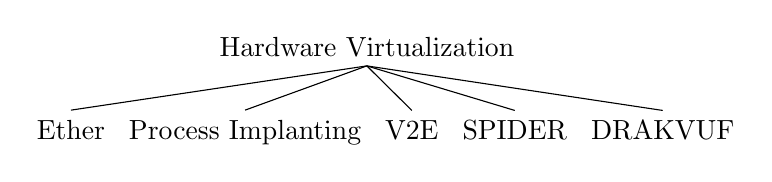
\begin{tikzpicture}	
		\Tree  
		[.Hardware\ Virtualization [.Ether ] [.Process\ Implanting ] [.V2E ][.SPIDER ][.DRAKVUF ]]
		\end{tikzpicture}
				\caption{Malware Analysis using Hardware Virtualization techniques}\label{tab:hardware-virtulization}
	\end{figure}


	
	\subsection{Static Malware Analysis}
	When we analyze software without executing it then that technique is called as Static Analysis. Similar concept is applicable when we perform analysis of malware. Static Analysis techniques can be used on the binary representation of a program. When we compile a program, certain information about the program gets lost and becomes deprecated. This loss of information makes it difficult to perform static anlaysis.
	There are certain ways, reverse engineers use in order to perform this static analysis of binaries. The well known tool IDA Pro~\cite{eagle2011ida}, is used to convert this binary into assembly code. This assembly code are raw instructions which execute at memory level. Hence, studying these is a very difficult task. Engineers also used inbuilt linux utilities like strings, gnu debugger~\cite{mercer2005model} to analyze this malware binary.
	Hence, it is important to develop automated techniques in order to overcome these difficulties. This is where researchers thought about executing a malware in a sandboxed environment and then analyze it. The sections throughout this article talk about these techniques and their strategies.
	
	
	\subsection{Dynamic Malware Analysis}
	Static analysis techniques like signature based anti-virus scanners to analyze and detect malware were widely adopted, but attackers devised methods such as code obfuscation, polymorphism and encryption of the malware to escape detection. Due to this reason, security vendors began using the runtime (dynamic) behavior of the system to detect malware. Several these systems have been used in practice today, but it is necessary to keep in mind several principles and attacker strategies that could be used to combat the dynamic detection of malware. We research several techniques that help in effective designing of systems that aid dynamic detection of malware and how efficient these techniques are on real-world malware samples.
		\subsubsection{Designing an effective Sandbox to detect Malware}
		Sandboxes are basically used to carry out automatic malware analysis by executing an unknown malware program in an isolated computing environment and then observing and analyzing it’s behavior. The paper [1] talks about building an effective sandbox that would help understand the malware behavior as deeply as possible and addresses the different responses from attackers and malware authors. For each of these responses the literature is researched in detail to understand how to combat these techniques of malware authors.

		According to [1], a good sandbox has the following three properties: Visibility, resistance to detection and scalability. When a malware is executed on a sandbox, every action of the malware should be visible to the sandbox to detect malicious behaviors. In this paper, different ways of monitoring malware execution in user mode is observed by the sandbox. Thus, the sandbox looks only at the system call interface and therefore is unable to observe the activity that happens in between the system calls. Thus, good sandboxes should have better visibility by also monitoring the program execution deeply by monitoring instructions in addition to just hooking the system calls. If a sandbox is detected by a malware program, it will alter it’s behavior which will make the malware sample difficult to be detected. This addresses the resistance to detection goal. According to the third goal, we should be able to run many samples of the malware on a sandbox without them interfering with each other and automatically.

		The paper then goes further to describe how a sandbox can be built, while maintaining the above three properties. Virtualization and Emulation are the two ways in which a sandbox can be built. An emulator basically simulates the complete hardware in the software. For example, an android program that is written for ARM can be run with the help of an android emulator on a x86 host machine. Hence, with the help of an emulation, detailed information of a running program can be obtained with the drawback that the performance of the software layer is low. In virtualization, parts of the computer hardware are simulated and while the guest program runs on the underlying hardware by occupying actual physical resources. This makes simultaneous running of virtualization software and the malware program impossible. The sandbox will be paused when the malware will be running and will only be alive during system calls. This makes detailed data collection difficult and detection of the virtualization software by the malware easy.

		By going the emulation way, an actual OS can be installed and run on top of an emulator. This serves the purpose by allowing the malware to execute in a real OS which makes it difficult for it to detect the analysis environment and a system emulator allows a sandbox to analyze every instruction executed by the malware program in addition to every access of the memory. But system emulation has two disadvantages that need to be overcome. The first one is that we need to understand the guest OS deeply in order to map the detailed view of the system to that in context of the guest OS. The second one is that methods like dynamic translation need to be adopted while analyzing the malware program to make emulation faster. While designing the sandbox using these ways, malware authors use several techniques to bypass detection. We explore two other literatures to understand these techniques.
		
		\subsubsection{Exploring Multiple Execution Paths to detect Malware}
		One technique that malware authors use to fight malware detection is environmental checks, i.e. the malware programs contain checks for the execution of certain parts of their code and if these conditions are not met while it’s interaction in that execution trace in which it is analyzed, incorrect conclusions may be drawn as these conditional parts of the code have not been executed. In this way, the malware will escape detection by the system. Also, if the malware detects the presence of a virtual machine environment using certain comparison checks, it will alter it’s behavior to escape detection. Some paths taken by the malware are also dependent on the time of the day, user IP addresses, presence of certain files and directories, reading content from network etc. For this reason, a more detailed view of the malware program execution is necessary. The paper [2] proposes a solution that addresses this problem and allows automated malware systems to explore multiple execution paths of a malware program, depending on how certain inputs are processed by the code. It tracks some interesting inputs that are read by the program and then identify decision points that use these inputs to decide the program flow. The decision points are then snapshot so that we return to them to alter the inputs in such a way that it explores all possible branches.

		When we take different execution paths we observe different behavior in each of them. The points where different branches are to be taken are selected on the way in which input is processed by each of the decision points before the branching starts. We identify the inputs of interest (filenames, time, directories etc.) and label these inputs so that whenever these inputs are encountered at a decision point, the system takes a snapshot of the process at that point so that we can return to this point to go along the other branches. To take the different execution paths, we need to rewrite the input values that were used in a control flow decision in such a way that the outcome of the decision is reversed. Now, the memory location corresponding to the control-flow decision must be updated. But only updating one memory location is not enough because the value at this location might have been copied in other locations in the subsequent process and used for many other calculations as well. Also, the choice of value for a given input must be such that all previous constraints on the input must be considered and we may even encounter times when there is no possible value of the variable that can be assigned to analyze the alternative path.

		Input can be tracked by assigning labels to related memory locations and by considering linear and non-linear dependencies between variables in the program. Using inverse mapping the addresses of the labeled memory locations can be stored so that simultaneous modifications of related memory locations is possible. When we come back to a program state to take an alternative path, the path constraint must be considered so that we do not create inconsistent states and reach impossible paths. In this manner, the labelled input variable will take values from the solution space that is created by the constraints. When multiple branching is encountered, depth-first search approach is followed to explore the execution space. Thus, in the paper these concepts are implemented by building the system on emulator QEMU. The execution state of the program (complete active memory content) is then stored into memory mapped pages and then the content of these pages is overwritten with the current state whenever we reset a process to take the alternative path. When the malware program is executing a particular branch, care needs to be taken that the process does not terminate, otherwise the old handles will not be valid and it would become impossible to return to a previous state. There may be cases of stalling code in a particular path due to certain endless loops, thus the system sets a timeout for every path (about 20 seconds) so that when the timeout expires, system waits to return to a safe state and then goes back to the snapshot to execute a different path. An optimization approach is implemented for string checking where if the first characters of the strings are different they are deemed unequal the first path is taken or if they are equal the second path is taken.  This optimization decreases significant overhead due to string comparisons at branching points.  

		This approach has several limitations. One of them is that when input is read from data collected from the network after establishing a connection; it is not possible to return back to a previous state as the connection will be lost. This tool also doesn’t have support for signals delivered to a process and multithreaded applications. Inspite of that, the malware analysis tool was run on 308 samples covering viruses, worms, Trojan horses and bots and for many these samples, it was observed that the system was exploring multiple paths. This prevents the bypassing of environmental checks and security vendors can improve their sandbox.
		
		\subsubsection{Bypassing stalling code that will prevent Malware Detection}
		Another technique used by malware authors to escape malware detection is by adding stalling code. This problem affects all the analysis systems alike. This is the code that executes, before the malware can perform any malicious activity, for a long enough time for the analysis system to tag the malware program as non-functional as the system will have limited time to execute a single sample. Also, the malware code is written in such a way that it takes more time to execute in a virtual analysis environment than it’ll take on an actual host. This is because, if the execution takes an unusually longer time, antivirus programs or attentive users may detect it. The paper [3] presents techniques to detect such stalling code. To satisfy the properties of stalling code, it is concluded that such type of code contains operations to slow down it’s execution and these slow operations are looped many times. 

		HASTEN is a dynamic analysis system that is proposed to detect stalling loops and ensure that do not affect analysis results of the sandbox. In the monitoring mode HASTEN observes all threads of the process to check of any of these have entered a stalling region. When this mode detects a slow-operating code HASTEN tries to identify the code region that executed repeatedly by recording the addresses of the instructions and building a CFG (Control Flow Graph) to search for loops. After such a loop is identified, this region of the code is whitelisted to allow detailed malware introspection as this could be a potential stalling code, while allowing the sandbox to continue its analysis. The CFG is analyzed to search for active loops and then several heuristics are applied to pick the loop that most likely has stalling code. The code parts that are reachable from the selected active loops are also marked as the stalling region. HASTEN then utilizes the CFGs to alter the execution of the program in such a way that the execution of the whitelisted region is skipped and enforcing the thread to continue execution along a path that Is outside of the stalling region. This might lead to inconsistent states. Therefore, whenever a variable from a whitelisted region is encountered outside of it, the program execution is halted and a correct value for this variable is determined using the tool Inspector gadget.

		HASTEN thus aims to reveal how a malware program with stalling loop would behave if it did not have any stalling code. Therefore, the malware samples were re-run twice by one run (redundancy run) using settings that would be utilized for base run of the sample and in parallel the test run using HASTEN was executed. If the test run reveals added features compared to the redundancy run, the redundancy run is compared to the base run. If the base and redundancy run differ largely, then the added behavior is independent of HASTEN else, the added behavior is the one that the sample will execute in the absence of stalling code. Only previously executed code is whitelisted, so there is no way in which the execution of a malicious code inside a code region that is marked stalling code will be skipped. 

		Analysis of 29,102 real-world samples twice; one with the redundancy run and the other with HASTEN shows that it can reveal additional behaviors in those samples that contain stalling code. 

		Ultimately, visibility of all instructions and ability to analyze and test by constructing a CFG and analyzing loops for activity is possible only when the sandbox can observe all the executing instructions. Thus, according to the literature building a sandbox that relies on virtualization alone is not enough as it does not offer enough insight into the behavior of a malware program and is an analysis platform that is able to analyze every instruction that a malware executes. This also allows resisting various actions that malware authors might take against malware detection.
		
		\subsubsection{Using BareCloud System to detect Malware}
		To understand more dynamic malware analysis techniques we research another literature that talks about BareCloud which is a dynamic automated malware detection system based on a bare-metal malware analysis technique. In this technique behavior of a sample in different analysis environments in compared to that in a reference system called a bare-metal. BareCloud basically analyses similarity in malware behavior in different systems using a hierarchical based approach. This tool extracts information of the malware behavior using disk and network level activity. It aims to identify the deviations in the dynamic behavior of malware when executed on a bae-metal reference system and other emulation and virtualization environments. The paper~\cite{kirat2014barecloud}, uses four such environments – Virtualization, Emulator, Hypervisor and Bare-metal on which malware is executed. The Scheduler synchronizes the execution of the malware sample in the different environments. The behavior of the malware on each of these environments is analyzed by the BareCloud system to detect malicious behavior.
		The four analysis environments are as follows:
		\begin{itemize}
			\item Cuckoo Sandbox~\cite{willems2007toward} – a virtualization environment supporting automated analysis and has components that can monitor execution related events in the analysis host. The behavioral profile of the malware is built using Windows API call traces and network traffic.
			\item Anubis platform []– Qemu[] based emulator that performs monitoring by observing how the pre-computed memory addresses, that correspond to system API functions, are executed. It also inserts it’s own instructions to the emulator instruction chain to gain additional information.
			\item Ether~\cite{dinaburg2008ether} – A Xen-based framework utilizing Intel’s VT hardware virtualization extensions. It provides the benefit of executing malware instructions as native CPU instructions on the real hardware as is. To build the behavior profile of malware system call traces and network traffic information is used.
			\item Bare-metal~\cite{kirat2014barecloud} -  A cluster of hardware-based modular worker units. It has a remote-control mechanism that helps automation of malware analysis on each of the worker units. The malware initiator which is used to start the malware execution removes itself and all its artifacts from the system once the initialization is done to escape detection by the malware.
		\end{itemize}
		The deviation in malware behavior in each of these systems is due to the change in activities performed by the malware after it is detected. For example, malware behavior might depend on any random value that it reads from its environment, it might depend on the presence of a software component or on it’s interaction with network devices. Effect of these factors needs to be minimized to effectively identify the deviations caused by evasive techniques of the malware samples. For this reason, the malware is simultaneously executed in all the environments using the scheduler. The external network devices that the malware instance interacts with are kept identical and all DNS and SMTP communications are intercepted so that consistent replies are given to queries by the different malware instances for each of the four environments. Out of the four analysis environments, from the first three, we extract the transient behavioral profiles that summarizes all the operations that a malware performs from the start to end. Such transient behavior can be obfuscated by the malware to evade transient behavior based similarity detection. But similar malicious activities result in the similar transient profiles irrespective of obfuscation. In the bare-metal environment we can obtain only the resultant behavioral profile due to transparency constraints. Comparison of disk contents from before and after malware execution can offer insight into the behavioral profile. During the extraction of a behavioral profile, only the objects and the operations carried on the objects are considered.
		Changes in the meta-data of the files and registry keys are considered to understand deviations in the objects before and after malware execution in the bare-metal system. For the first three analysis systems, system call traces are analyzed to extract the behavior profiles. Now the behavior profiles that correspond to malware execution only, are filtered by different methods like understanding the behavior of the base OS and filtering it from the profile that is generated by malware execution. Hierarchical similarity based approach is used to compare the behavioral profiles. A hierarchy is represented in the form of a tree where the first level of similarity is an object type (root) which can one or more objects associated with it and each of these objects can have one or more operations associated with them. Each operation can have one attribute (leaf) associated with it. To compute the similarity, we first identify the matching nodes in the trees of two behavioral profiles starting from the root of each and reaching to the leaves. The similarity at each level is calculated in the first step and in the next step similarity at each level is aggregated to obtain the overall similarity. The behavior deviation score between the various profiles for a malware sample calculated with reference to the bare-metal behavioral profile obtained from the bare-metal analysis system, is the quadratic mean of the behavior distances that are obtained directly from the similarity distances. The deviation score is in the interval [0, 1] and a deviation threshold is defined. If this threshold is exceeded, the sample is considered as evasive.  

		All the known and unknown fingerprinting techniques that are used to detect virtualization and emulation platforms will fail to detect BareCloud as malware is being executed on a bare-metal environment – this is the biggest advantage that this system provides over previous methods. Also, it incorporates hierarchical similarity technique that computes similarity on the element-level rather than on the profile-level by encoding knowledge of events occurring at every level. Inability to handle stalling code and environment detection due to heuristic checks employed by malware to search for anomalies are some of the disadvantages of BareCloud.
		
		\subsubsection{Automatic Extraction of Evasion Signatures in Malware}
		The technique presented in ~\cite{kirat2014barecloud} for malware detection needs a malware analyst to reanalyze a malware sample to understand the technique used for evasion. This consumes a lot of resources and is not scalable. Thus, the paper ~\cite{kirat2015malgene} presents MALGENE which automatically extracts the evasion signatures from the malware behavior in system call sequences using data mining and data flow analysis techniques. The call events and data comparison events are used to construct concise signatures and then eventually group them into different evasion techniques. MALGENE utilizes the tool BareCloud~\cite{kirat2014barecloud}  for information on malware evasion and carries out its further analysis.
		Malware escapes analysis by gathering information about its environment and then performing some comparisons and calculations on the gathered information to decide whether to evade or not. This information consists basically of system call events, user API call events and comparison events that eventually forms the evasion signature. The sample is analyzed in two different execution environments, one in which it evades and shows malicious activity in the other. The system call sequences of the two samples are aligned and checked for deviation. The point of deviation represents the evasion point. This is where the sample performs it’s evasion check from where the evasion signature is extracted. All the strategies given in ~\cite{kirat2014barecloud} to avoid deviations caused by external factors are taken care of. Sequence alignment algorithms from bioinformatics are used for checking deviations in the sequence alignments. Global Alignment and Local Alignment approach are used to sequence the alignment. The global alignment algorithms compare the entire subsequences and therefore the alignment spans the entire length of the subsequence, whereas the local alignment finds matches of local subsequences in the two subsequences. The local approach is better when there are large missing parts in the sequence. Finding a similarity score between the subsequences is one of the important parts to understand match and mismatch of system calls. Importance of arguments associated with system calls, importance of alignment of some system calls over the others and many other factors lead to the proposal of a similarity scoring schema to calculate the similarity between two system calls. Also, the gap penalty schema is decided to calculate the gap penalty score which helps identify gaps introduced by evasion. Repeated short subsequences due to looping are discarded if they repeat more than five times.
		An evasion section is chosen consisting of system calls, API calls and comparison events before the evasion point. The inverse document frequency metric is used to filter out the call events from the evasion section that are too frequent in non-evasive malware. The Anubis emulator is used to generate the execution profile of the malware and the system call sequence is extracted from the environment that the malware has evaded. The comparison events are then extracted from the evasion section and the call events filtered using inverse document frequency represent the final evasion signature. These evasion signatures are then hierarchically clustered using complete-linkage method and Jaccard similarity.
		The limitation of the approach is that due to the requirement of system call sequences from the analysis environment we cannot use bare-metal execution. This technique was evaluated on 2810 evasive samples and by extracting the evasion signatures, it grouped the samples into 78 evasion techniques. Thus, MALGENE allows us to extract evasive signatures from evasive malware that could be used to prevent evasion of malware from dynamic detection systems.
		
		\subsubsection{Detect Malware Based on API Call Sequence Analysis}
		The authors of ~\cite{ki2015novel} propose a novel approach for the dynamic analysis of malware. We embrace DNA succession arrangement calculations and concentrate normal API call grouping examples of malevolent capacity from malware in various classifications. We find that specific malignant capacity are usually incorporated into malware even in various classifications. From checking the presence of certain capacities or API call arrangement designs coordinated, we can even identify new obscure malware.
		
		As a conclusion we make a tree structure of various techniques employed by Dynamic Malware Analysis. This can be described as Figure~\ref{Dynamic}
		\begin{figure}
			\centering
				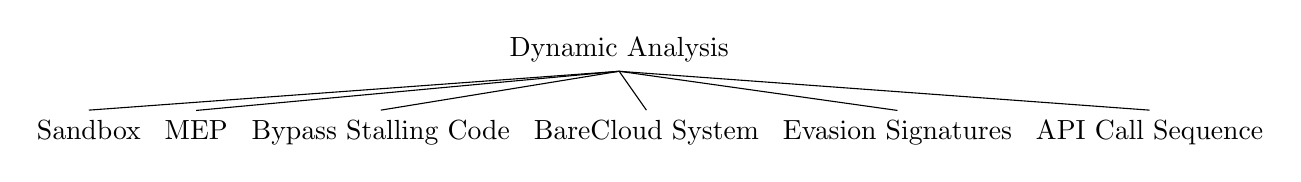
\begin{tikzpicture}
			\Tree
			[.Dynamic\ Analysis [.Sandbox ][.MEP ][.Bypass\ Stalling\ Code ][.BareCloud\ System ][.Evasion\ Signatures ][.API\ Call\ Sequence ]]
			\end{tikzpicture}
			\caption{Dynamic Malware Analysis Techniques}\label{Dynamic}
		\end{figure}

	\subsection{Malware Reverse Engineering}
	In the literature survey below we will be exploring concepts like malware reverse engineering and the common terminologies used, the advantages of automatic reverse engineering etc. We will start off by exploring the current industry leader in decompilation i.e. Hex-Rays and its enhanced versions like DREAM~\cite{yakdan2015no} and DREAM++~\cite{yakdan2016helping}. We will also be diving deep into the working of some of these state-of-the-art decompilers~\cite{guilfanov2008decompilers} and the techniques used by them. Further , we will expand our scope and see how honeypots can be leveraged to perform reverse engineering and lastly we will try to understand how attackers obfuscate their malware which makes decompiling them harder and how we can reverse engineering such malwares. We now proceed to talk a bit about decompilers and how they can aid in malware reverse engineering and if they are better than dissassemblers/debuggers.\\ \\
	
	A malware is a program which is hostile to the environment its deployed on. These malwares are typically deployed by an attacker who wants to harm the systems. The only trace of the malware on the host system is the malware itself(the binaries/ executables). In order to build a defense layer to prevent such attacks in the future we need to know what the malware exactly does. Hence the process of converting an executable to its source code is very important and this is what a decompiler does. Programs are binary applications and their working can be found out from what OS level activities are going on in the system, keeping a track of all the changes and making calculated guesses as to what the instruction would look like from a higher level of abstraction. We can even use a disassembler which can convert the malware to its assembly level code but it makes the life of the analyst/ reverse engineering much harder as they have to mentally map this lower level of abstraction to higher level. IDA Pro is an example of such a disassembler. Building a robust decompiler is next to impossible and even the best ones will have some imperfections but we can try to mitigate that as much as possible.The basic phases of a good decompiler are given below. Hex-Rays is built using the same concepts more or less.
	\begin{enumerate}
		\item Microcode generation : Checks if all the functions are well defined
		\item Local optimization: Simplifies instructions
		\item Global optimization: propagates expressions, removes dead code
		\item Local variable allocation: variable ranges and size are determined
		\item Structural analysis: Control flow graphs are created and analysed
		\item Pseudo Code generation: based on microcode and structural analysis steps the output file is generated
		\item Pseudo Code transformation: Transform the output to make it look more readable
		\item Type analysis: Analyzes pseudocode, builds type equations
		\item Final touch: Rename variables etc.
	\end{enumerate}
	In the next few papers we will research on other decompilers like DREAM, DREAM++ and other concepts and tools relevant to malware reverse engineering.
	
		\subsubsection{DREAM}
		
		Decompilation is an essential part of malware reverse engineering as it helps to automate the tiresome process. But the decompiled code should be meaningful and should be highly structured. The typical decompiler relies on the control flow graph and tries to generate a structure for the malware program. If the decompilers do not find any mapping it generates a GOTO statement thus breaking the structure which makes the code hard to read for the analysts. DREAM is a software which produces a GOTO free code and maintains the code structure and is the first one to do so effectively . The software has also been compared to the leading industry decompilers like Hex-Rays and Phoenix and also produces a more compact code which makes it easily understandable to the one’s trying to figure out what the malware actually does. The author proposes a technique called pattern-independent control flow structuring which is based on the following two intuitions:
		\begin{itemize}
			\item A single point of entry and a single point of successor for every high level construct
			\item A nested code construct can be identified when the logical conditions reach the Control Flow Graph(CFG nodes)
		\end{itemize}
		If there are multiple points of entry and successors then the decompiler tries to transform them into equivalent single entry/successor points. Abstract Syntax Tree(AST) and Control Flow Graphs are techniques of representing high level code and form the basis for performing  structural analysis. The way structural analysis works is that it recurses through the CFG and matches subgraphs to the stored patterns of high level code. If a match is found then the corresponding tree is collapsed otherwise a GOTO statement OS generated. This paper solves the problem of removing the GOTO statements by restricting the set of structured constructs sequences , conditions, loops and switch nodes. The following steps or phases describe the working of the DREAM decompiler:
		\begin{enumerate}
			\item First Stage: Binary file is parsed and converts the code to an intermediate representation
			\item Second Stage: Data flow analysis steps like eliminating dead code and constant propagation happen in this stage
			\item Third Stage: Inferring the variables happens at this stage
			\item Fourth Stage: This stage recovers the high level constructs from CFG which involves Control Flow Structuring and Post-structuring optimizations
		\end{enumerate}
		The first three stages use the existing standards, the fourth stage is what the paper focuses on and it gets segregated into two phases:
		\begin{enumerate}
			\item Pattern-independent structuring \& Semantics preserving transformations: This phase focuses on creating the abstract syntax tree (AST) and transform regions having multiple entries/successors into equivalent single entry equivalents
			\item Post-structuring optimizations: After the AST gets generated , this phase tries to optimize the generated constructs to improve code readability.
		\end{enumerate}
		The research on this area is extended by a team which devised the DREAM++ software which is built on DREAM and is a superior decompiler. In the next section we will study nuances of DREAM++ and the add-ons it provides to DREAM software.
		
		\subsubsection{DREAM++}
		Though decompilation is helpful, the current state-of-the-art decompilers produce complex code and do not efficiently perform the task of reverse engineering due to which the analysts have to frequently have to go back to debugging the assembly level code. The authors are trying to maintain the semantics of the code and thus produce a more user-readable code from the binary files which will help analyze malware more efficiently. The authors have come up with DREAM++ which is a usability-optimized decompiler and an extension to the current state-of-the-art decompiler DREAM. The paper gives a comparative study of DREAM++, DREAM and Hex-rays which the current industry leader decompiler and how DREAM++ stacks up against the two.\\ \\
		The authors started of by researching the already existing state-of-the-art decompilers like DREAM and Hex-Ray and conducted several interviews with the malware analysts already using them. This helped them understand the existing shortcomings of the softwares which would negatively impact the code readability. The main issues identified by the authors were:
		\begin{itemize}
			\item Complex Expressions: The decompilers usually produced more complex expressions than they actually were
			\item Convoluted  Control flow: the code produced contains complex sequencing flow
			\item Lack of high level semantics: the decompilers weren’t able to capture the semantics of variable names
		\end{itemize}
		The authors created DREAM++ by handling all these issues which would preserve the semantics of the malware code and improve readability. They also introduced a new metric for evaluation purposes called the "human factor" and evaluation studies were conducted to compare the three decompilers. The paper achieves two major contributions. First, the authors provided several code transformation technique which preserve the semantics to the malware code and improve code readability. The authors created DREAM++ an extension to the current state-of-the-art decompilers which simplifies expression and control flow transformations and also maintains the semantics of the variables and constants according to the context they were used in. Second, the authors conducted several studies to compare the three decompilers and note the improvements of the DREAM++ over the already existing decompilers. Reverse engineering binary files and preserving the semantics of the source code is a really challenging job. The authors have focused on code transformations for that but in my opinion there is a lot more to analyze in the code than only the three categories mentioned in the paper. The inclusion of a "human factor" metric is a really good idea as most of this research is done to eliminating manual reverse engineering. Besides the user studies were conducted on a handful of students and malware analysts which do not give an overall picture to the comparative study.
		
		\subsubsection{REWARDS}
		
		Automatic decompiling of code has always been a challenge as it is hard for automated softwares to determine the syntactic and semantic definitions of malwares just based on their executables. Here we define a technique called REWARDS~\cite{lin2010automatic} which will help us determine what data structures the malware is actually using. It makes use of the memory access patterns of the program, for example it tags/ attaches a timestamp with every location that is accessed and uses this parameter to predict the data structures that would have been used. An overview of the REWARDS tool is given below:
		\begin{enumerate}
			\item It is a technique for exposing the data structures given the binaries and is based on dynamic analysis.
			\item Executes the binary, observes the execution, gathers runtime information.
			\item Performs analysis and recovers the syntax and the semantics of the underlying data structures.
			\item REWARDS tries to infer the primitive data types such as char, float etc. and the semantics of program variables.
		\end{enumerate}
		REWARDS technique makes use of type sinks i.e. an execution point in the program where one or more variables can be directly resolved. These type sinks can be classified as:
		\begin{itemize}
			\item System calls: REWARDS can extract the type of arguments passed to system calls as the programs generally use the OS services via system calls
			\item Standard library calls: REWARDS can easily find the arguments of a well defined API call. These types of calls provide more information than the system calls and hence qualify for an ideal type sink
			\item Type-revealing instructions: Machine instructions can serve as type sinks as well
		\end{itemize}
		REWARDS uses an algorithm called the online type propagation \& resolution algorithm which exposes the variable types both syntactic and semantic ones sing type sinks. The end result of this algorithm is a printed file of all the variables and the memory location used. Most variables can be identified using this algorithm but some variables are freed during the execution and these variables make their ways to the log files. An offline resolution strategy is implemented to resolve such freed memory locations. The last phase of the REWARD technique is that it has to construct a hierarchical map of the memory locations that were accessed during the program's execution. The working is as follows:
		\begin{enumerate}
			\item Type all the top level global variables which forms the root section
			\item The variables form the leaf nodes and the edges in between are offsets, primitive type etc.
			\item If the leaf node itself is the pointer then the algorithm recurses through the sub tree
			\item Continue till no leaf node is a pointer
		\end{enumerate}
		REWARDS is widely used in fields like Memory Image Forensics and Vulnerability Fuzz.
		
		\subsubsection{HERESy}
		“Honeypots are networked computer systems specially designed and crafted to mimic the normal operations of other systems while capturing and storing information about the interactions with the world outside and are crucial technology in the study of cyber threats and attacks that propagate and occur through networks”~\cite{honeypot2016}.\\ \\
		This paper discusses how  honeypots are enhanced to perform reverse engineering activities and help in analysing the captured malwares. Typically honeypots are systems with low levels of protection which draws the attackers towards them. The current honeypots have low interaction functionality in the sense that most of them deploy emulated services. These honeypots are not as effective as its hard to study how malware propagates through such a system and also the smart attackers can identify such devices and easily by pass them. The crux here is to create a high interaction honeypot which can replicate the functionality of a real world system thus confusing the attackers so that they can completely show the malware’s behaviours and also adding the functionality of reverse engineering can help the malware analysis process on such honeypots. We learn about the working and architecture of HERESy a modular honeypot system which works at different levels of the honeypot system. The following steps describe the working of HERESy:
		\begin{enumerate}
			\item HERESy creates separate isolated working environments(containers) for every attacker/malware
			\item It tracks all the activities of the malware in logs and storage systems
			\item The containers are built on the fly when requests are made to services which are hosted on the honeypot
		\end{enumerate}
		The HERESy architecture leverages several modules and each is given a specific task during the hijacking process. The following is a list of modules used:
		\begin{itemize}
			\item Proxy Module: this module is in charge of creating separate containers for every incoming attacker/malware. It tracks the port to which the malware made the request to and routes all related requests to the container
			\item File System Module: Changes to the files on the honeypots file system are tracked by this module. It leverages the version control systems like git to track the file changes
			\item Network Module: This module performs the traffic analysis and is also referred to as the network sniffing module
			\item Process Execution Module: this module keeps a track of all the executables that the malware or the attacker downloads
		\end{itemize}
		
		
		
		\subsubsection{Rotalum`e}
		
		We will now talk about Rotalume~\cite{rotalumegatech}, a tool to perform automatic malware reverse engineering of malware emulators. Attackers are becoming smart and are finding new ways to stop security experts and analysts from decompiling and reverse engineering their code. As we saw in the discussions above it is very much possible to generate the source code given the binaries of the malwares. To stop this the attackers have started compiling their program to an intermediate bytecodes which are written in randomly generated instruction set. These programs are then paired with their native binary emulators which are able to correctly interpret the bytecode. In this section we focus on how we can reverse engineer such malware emulators.\\ \\	
		The obfuscators or the bytecode generation technique is similar to that of the execution of a java program. Instead of the Java virtual machine here we have emulators which can be built by the attackers and he/she is free to choose the semantics of the bytecode  instructions. For understanding and decompiling the source code we need to understand what the emulator does which in turn brings us to understanding the reverse engineering strategies. The typical static analysis like symbolic execution of the malware will be that of the emulator and not the actual source code of the malware. Both pure static and pure dynamic analysis fail to decompile the malware. There is a middle spectrum which includes techniques like dynamic tainting, information flow analysis and other instruction level analysis. These techniques analyze the emulators and not the malwares.\\ \\	
		We will now describe how the reverse engineering of emulators takes place. The emulated malware is executed once in protected environment and the entire x86 instruction trace is recorded. The bytecode’s syntactic and semantic information is revealed by the trace. The authors have come up with an algorithm which would give the behaviour of the unknown bytecode based only on reverse engineering the malware emulator. The algorithm is as follows:
		\begin{enumerate}
			\item Variables in the raw memory are identified from how they were accessed during reads and writes
			\item Narrow down on a subset of these variables that could possibly hold the programs Virtual program Counter(VPC)
			\item The boundaries of the bytecode data are found
			\item The syntax and  the working of the bytecode program is identified and how the emulator accesses the bytecode is also examined in this step
		\end{enumerate}
		
		\subsubsection{COBRA}
		Fine-grained ~\cite{vasudevan2006cobra}malware analysis is the task which enables the building of a blueprint of the malware core structure and functioning, that aids in the detecting and countering the malware and its variants. It can be accomplished by using both static and dynamic methods. This paper talks about one such dynamic malware analysis tool called Cobra.
		The paper begins by talking about what malware is and goes to explain the pros and cons of the static and dynamic approaches to fine-grained malware analysis in detail. The dynamic approach was set to be preferred as it allowed to detect malware while the code base is running so that the malware can be detected before the code changes into a version that contains more alterations than the original one. It also elucidates the various differences between coarse and fine grained approaches to malware analysis and begins to talk about Cobra as being superior to all existing dynamic malware analysis tools.
		Cobra~\cite{vasudevan2006cobra} is a dynamic fine-grained malware analysis framework that overcomes the shortcomings of current research in dynamic fine-grained malware analysis by providing a stealth supervised code execution environment that can handle multithreading, SM-SC code and any form of code obfuscation in both user- and kernel-mode. 
		Fine-grained malware analysis using Cobra is facilitated by a technique that we call stealth localized executions. The basic idea involves decomposing a code-stream into several groups of instructions which we call blocks that are then executed, one at a time, in a fashion so as to mimic the normal execution of the target code-stream. Each block is implanted with various invisible Cobra specific code constructs (as applicable), ensuring that the framework has complete control over the executing code-stream while remaining stealthy.	
		The framework core consists of: A Block Create and Execute Engine (BCXE), a disassembler, a block repository, a block-monitor, and a framework API. The design and implementation of Cobra is twofold. First, it should be able to provide a stealth supervised environment for fine-grained analysis of executing malware code-streams, supporting multithreading, self-modifying code and any form of code obfuscation in both user- and kernel-mode on commodity OSs. Second, one must be able to deploy the framework dynamically and selectively on malware specific code-streams while allowing other code-streams to execute as is. 
		This is achieved by the employment of:
		\begin{enumerate}
			\item Localized-executions: Cobra decomposes a target code-stream into several groups of instructions and executes them in a fashion so as to mimic the code-stream’s normal execution. This process is what is called localized-executions and the instruction groups are called blocks.
			\begin{itemize}
				\item Block creation: Cobra’s BCXE is responsible for creating blocks from the target code-stream and executing them. The BCXE employs an architecture specific disassembler on the target code-stream, to discover instructions one at a time, and create the corresponding blocks. Every block ends with a framework specific set of instructions — which is called a Xfer-stub that transfers control to the BCXE.
				\item Xfer-stubs: These are Cobra specific code constructs that terminate every block, can be abstracted as a function that takes a single parameter (Figure 3a). The parameter is an index into a Xfer-table, an internal data structure of the framework which enables the BCXE to obtain runtime information on the supervised code-stream.
				\item Obfuscated Code and SM-SC Code: Cobra’s model of employing xfer-stubs for every CTI (unconditional or conditional) enable the framework to support any form of code obfuscation, since obfuscated code rely on conditional and/or unconditional branches in between instructions for their functioning.
				\item Block Execution: Localized-executions start from a user-defined point — which we call an overlay point in a target code-stream. An overlay point is the memory-address (typically a OS and/or a library function address) in a target code-stream from where fine-grained analysis is desired.
				\item Events and Callbacks: Cobra generates various events during block execution. An analysis tool employing Cobra can employ event specific processing by registering callbacks functions to which control is transferred by the framework to process a desired event during block execution.
			\end{itemize}
			\item Stealth Techniques: Cobra employs a host of techniques to tackle issues involving privileged instructions and the framework stealthness. 
			\begin{itemize}
				\item Stealth Implants: Cobra scans a block for privileged instructions and instructions that betray the real state of the executing code-stream and replaces them with stealth-implants which Cobra code constructs that aid in supervised execution of privileged instructions and the framework stealthness, while preserving the semantics of the original instructions in the target code-stream
				\item Cloning: Cobra uses a technique called cloning to hide the framework while at the same time allowing the malware to access such critical structures. The framework maintains a copy of critical memory regions such as the page tables/page-directories, IDT, GDT etc. The framework block-monitor tackles issues such as reads and/or writes to such critical structures by presenting the clone of these memory region.
			\end{itemize}
			\item Skipping and Block-Coalescing: Execution of blocks under Cobra involve control transfers to and from the BCXE. These transfers result in the saving and restoration of the processor registers which contribute to the framework latency. Cobra employs a technique that we call block-coalescing to minimize latency due to such code constructs. In this technique, a group of blocks are brought together to form a single block, preventing multiple control transfers to the BCXE.
			\item Framework API: Analysis tools that employ Cobra are usually written in C/C++ using the framework API. The API is easy-to-use and is designed to be platform independent whenever possible allowing tool code to be re-usable while allowing them to access platform specific details when necessary.
		\end{enumerate}	
	Performance measurements of the framework using Wildcat under various environments were made, by which the latency effects were noticed. It was concluded that the nature of the code analyses and the style used in terms of the ranges selected and the coalescing blocks determine the latency one might expect and even the worse possible latency was found as acceptable.
	In this paper, the authors presented Cobra: a stealth, efficient, portable and easy-to-use dynamic fine-grained malicious code analysis framework that overcomes the shortcomings in current research involving fine-grained code analysis in the context of malware, while not making any visible changes to the executing code and hence not being detected or countered.
		\subsubsection{MEF}
		MEF~\cite{schultz2001mef} is a malicious email filter that scans windows attachments for malware by integrating with a UNIX mail server. It is seen as attachment to the existing Procmail’s filter such that the virus scanner system can be avoided, where only the known malware can be detected. Instead, the email is scanned when it is received by the source to detect unknown malware and give warnings and or block the message. 
		The goal of this paper is to describe a data mining based filter which integrates with Procmail’s pre-existent security filter to detect malicious executables.

		MEF filters malicious attachments by replacing the signature based virus filter found in Procmail with a data mining generated detection model. Procmail is a program that processes email messages looking for information in the headers or body of each message, and takes actions based on what it finds. The filter first decodes each binary and then examines the binary using a data mining classifier. It evaluates the attachment by comparing it to all the byte strings found with it to the byte-sequences contained in the detection model. The system calculates the probability of the binary being malicious, and if it is greater that its likelihood of being benign then the executable is labeled malicious. Otherwise, the binary is labeled benign. This is reported as a score back to Procmail, and then is used to either send the mail along untouched, or the entry is logged as the attack and email is wrapped with a warning.
		Borderline binaries are binaries that have similar probabilities of being benign and malicious (e.g. 50\% chance it is malicious, and 50\% chance it is benign). The binaries are important to keep track of because they are likely to be mislabeled, so they should be included in the training set. To facilitate this, the system archives the borderline cases, and at periodic intervals the collection of borderline binaries is sent back to a central server by the system administrator. Once at the central repository, these binaries can then be analyzed by experts to determine whether they are malicious or not, and subsequently included in the future versions of the detection models.

		The MEF system will require updates periodically. After a number of borderline cases have been received, it is necessary to generate a new detection model, and subsequently distribute updated models. A new model is first generated by running the data mining algorithm on the new data set that contained the borderline cases along with their correct classification, and the previous data set. This model will then be distributed. Updating the models is accomplished by distributing portions of the models that changed, and not the entire model.

		Monitoring the Propagation of Email Attachments works by having each host that is using the system log all malicious attachments, and the borderline attachments that are sent to and from the host. This logging may or may not contain information about the sender or receiver depending on the privacy policy of the host. In order to log the attachments, there is a need for a way to obtain a unique identifier for each attachment. This is done by using the MD5 algorithm to compute a unique number for each binary attachment. The input to MD5 was the hexadecimal representation of the binary. These identifiers were then kept in a log along with other information such as whether the attachment was malicious, or benign and with what certainty the system made those predictions. The logs of malicious attachments are then sent back to the central server according to the policy of each host. After receiving the logs, the system measures the propagation of the malicious binaries across hosts. From these logs it can be estimated how many copies of each malicious binary were circulating the Internet, and these reports will be forwarded back to the community, and used for further research.
		The data mining detection model involved using a large dataset consisting of both malicious and healthy attachments and converting them into hexadecimal by using the hexdump[5] tool.
		The classifier that was incorporated into Procmail was a Naïve Bayes classifier [5]. A naive Bayes classifier computes the likelihood that a program is malicious given the features that are contained in the program. The model output by the naive Bayes algorithm labels examples based on the byte strings that they contain. For instance, if a program contained a significant number of malicious byte sequences and a few or no benign sequences, then it labels that binary as malicious. Likewise, a binary that was composed of many benign features and a smaller number of malicious features is labeled benign by the system. The naive Bayes algorithm computed the probability that a given feature was malicious, and the probability that a feature was benign by computing statistics on the set of training data. Then to predict whether a binary, or collection of hex strings was malicious or benign, those probabilities were computed for each hex string in the binary, and then the Naive Bayes independence assumption[5] was used. The independence assumption was applied in order to efficiently compute the probability that a binary was malicious and the probability that the binary was benign.

		The results of this methodology was compared with a signature based approach where unique identifiers were constructed for each malware and the overall result showed 96\% accuracy while using the data mining method and 49\% accuracy while using the signature based method. However the false positive rate was the lowest for the signature based methodology. When using known executables the data mining method had a 98\% approx. accuracy in detection rate whereas signature based method was at a 100\% accuracy. 
		The advantages of this data mining method is that new malicious malware is found due to the data mining nature of the algorithm, lower amount of resources in terms of RAM and CPU are used and also low false detection rates by further training the system with the borderlines.

		\subsubsection{OmniUnpack}
		OmniUnpack~\cite{martignoni2007omniunpack} is a tool that monitors the execution of a program and the removal of the layers one by one to find the malware packed underneath. It directly provides the malware to the detector and with the increasing in the percentage of new malware packed from 20\% to 80\%.
		OmniUnpack is seen as a generalized unpacking algorithm to eliminate custom routines to be defined for each packing algorithm found in the programs. This malware detector is resilient to anti debugging and integrates with any operating system without reducing its efficiency and it is also independent of packing and self modification.
		The detector works by monitoring the memory access of the program at a page level and is employed when data is written to the memory and is then about to be executed but the problem of determining when the unpackingI[3] is finished is difficult. The paper also talks about dangerous system calls that could be the malware communicating with the host and this is monitored by OmniUnpack as well.
		The algorithm that is used follows a simple strategy to handle packed code. All memory writes and the program counter are tracked. If the program counter reaches a written memory address, we know that some form of unpacking, self-modification, or code generation occurs in the program. All written-then-executed (or written-and-about-to-be-executed) memory locations should then be analyzed by a malware detector.	
		An execution trace of the program can be divided into four different stages, one per unpacking routine and one for the original code.
		OmniUnpack monitors the execution of the program and records the memory locations that were written and, of those, the memory locations that were written and then executed. As long as there are no memory locations that are written and executed, there is no reason to invoke a malware detector. If a memory location is written and is about to be executed, it is a candidate for malware detection.
		The OmniUnpack Algorithm:	
			The algorithm ensures that every code fragment reached during a program execution is checked by a malware detector before the host system might be irreparably harmed. The OmniUnpack algorithm monitors the execution of the program and invokes the malware detector on newly generated code. The program is stopped while the malware detector is executed and resumed if no malicious code is found.
			The algorithm tracks the memory pages that were written(the set W) and the memory pages that were written and executed (the set WX). Obviously, WX⊆W. When the program invokes a dangerous system call after executing code from a previously written memory page(line 11), the algorithm triggers malware detection on all the pages written (i.e., those recorded in the set W). Unless the process is found to be malicious and thus terminated, the system call is allowed and execution is resumed.

		Implementation:
		OmniUnpack is implemented as a kernel driver for Windows XP.
		The system is composed of a kernel driver and a user-space component. The kernel component is responsible for tracking memory accesses to detect the end of an unpacking stage detecting when a dangerous interaction between the suspicious program and the system occurs triggering malware detection. The user-space component consists of a malware detector responsible for on-demand scanning of memory of the suspicious program. The kernel component keeps track of the memory locations that can potentially contain newly generated malicious code.

		Monitoring memory access is implemented by leveraging the memory protection mechanism offered by the hardware. When an unpacking routine writes the unpacked code to memory, the destination page is marked as writable but not executable. At the end of the unpacking stage, when the program accesses the same page for execution, the lack of execution permission causes a protection exception that is reported to the operating system (OS). Such exceptions are intercepted and processed.
		Monitoring system calls is done through interposition on the system-call dispatch table. If newly generated code is present in the program memory, the code is executed, and the execution is followed by a dangerous system call, we consider the unpacking stage concluded and we trigger malware detection. The system call is consequently allowed only if no malicious code is detected.
		OmniUnpack provides a user space Malware detector with data to analyze and then authorizes, or denies, the execution of such data according to the response of the detector. If the detector adopted fails to identify the presence of malicious code in memory, the system will resume the execution because the response of the detector is assumed to be correct. The advantage of running the malware detector in user-space is that a bug in the malware detector will not compromise the stability of the whole system. Before Invoking the user-space detector, the kernel component maps in the virtual address space of the malware detector process, the pages for which the analysis is required and communicates to the detector the address and the amount of data to analyze. The malware detector then scans the memory region part of its address space. The detection is triggered during the execution to scan only the pages that potentially contain the newly generated malicious code. Therefore, pages executed without prior modification do not trigger detection.
		Experiments showed that the execution time of OmniUnpack was far lesser than that of its counterparts such as PolyUnpack and ClamAV.It also handled about 80\% of the malware as compared to the other two applications.Also the overhead for the application was seen to significantly lesser than its counterparts.
		
		\subsubsection{Fileprints: Identifying File Types by n-gram Analysis}
		This paper talks about the application of n-gram analysis to the training files to produced n-gram distributions that represent all the files of a specific type.  A Fileprint~\cite{li2005fileprints} is the representation of the full 1-gram distribution of all members of a single file type of file almost like a histogram. This fileprint is unique for HTML,ZIP,DOC, PDF files etc. It can be used to check security policies, type of data carried and also if any infection is there as this will alter the fileprint of the file.
		An application of n-gram analysis: Infected file shares may be detected if they do not conform to an expected file type distribution. Hence, virus and worm propagation may be thwarted if certain files do not match their announced type. n-gram analysis of file content was first proposed for the detection of malicious virus code in emails where, a supervised training strategy was applied to model known malicious code and detect members of that class in email attachments. The n-gram distributions that were used as input to a supervised Naïve Bayes machine learning algorithm to compute a single classifier of “malicious file content”. In this paper, the authors extend these techniques by calculating the entire 1-gram distributions of file content and use these as models for a set of file types of interest. The distribution of byte values of a file are compared to the models using well known statistical distribution distance measures (Mahalanobis and Manhattan distance) \cite{li2005fileprints}. 
		An n-gram is a subsequence of N consecutive tokens in a stream of tokens. By converting a string of data to n-grams, it can be embedded in a vector space to efficiently compare two or more streams of data. Alternatively, we may compare the distributions of n-grams contained in a set of data to determine how consistent some new data may be with the set of data in question. An n-gram distribution is computed by sliding a fixed size window through the set of data and counting the number of occurrences of each “gram”. In this paper, 1-gram analysis is considered.
		Given a training data set of files of type A, we compute a model MA. For each specific observed file, MA stores the average byte frequency and the standard deviation of each byte’s frequency. Once a model has been computed, we next consider the comparison of a test file against this model, either to validate the file’s purported type, or to assign a type to a file of unknown origin. We use Mahalanobis Distance for this purpose. Mahalanobis Distance weights each variable, the mean frequency of a 1-gram, by its standard deviation and covariance. The computed distance value is a statistical measure of how well the distribution of the test example matches (or is consistent with) the training samples, i.e. the normal content modeled by the centroids. This way, A malware detector would require us to build a set of models for a set of expected file types.
		Some commonly used strategies to increase the efficiency and accuracy of the modelling technique are:
		\begin{itemize}
			\item Truncation: Truncation simply means we model only a fixed portion of a file when computing a byte distribution. For most files, it can be assumed that the most relevant part of the file, as far as its particular type, is located early in the file to allow quick loading of meta-data by the handler program that processes the file type. This avoids analyzing a good deal of the payload of the file that is not relevant to distinguishing their type and that may be similar or identical to several different file types.
			\item Multiple Centroids: files with the same extension do not always have a distribution similar enough to be represented by a single model. clustering strategy. Rather than computing a single model MA for files of type A, we compute a set of models MkA , k>1.The multiple model strategy requires a different test methodology, however. During testing, a test file is measured against all centroids to determine if it matches at least one of the centroids. The collection of such centroids is considered a fileprint for the entire class. The multiple model technique creates more accurate models, and separates foreign files from the normal files of a particular type in more precise manner. In this paper, the multiple models are computed by the K-Means algorithm under Manhattan distance.
		\end{itemize}
		The experiments that were performed utilized 2 groups of data sets, each containing different file types and during computation some of them seemed to have very similar 1-gram distributions. Only files of similar size were compared as well. Next the entire and truncated files were used to find out how well they file type could be identified by the fileprint. It turned out that very few files were misclassified while using truncated files in a one-centroid file type model accuracy. Next multi-centroids file type classifying techniques showed better results with almost a 6-7\% increases for certain truncation sizes. Finally each file was tested against the distribution of randomly chosen set of exemplar files and the general consensus was that the results in terms of average accuracies was better than the previous two methods.\\
		As a conclusion we make a tree structure of various techniques employed by Malware Reverse Engineering. This can be described as Figure~\ref{Reverse}\\
		\begin{figure}[t]
			\centering
				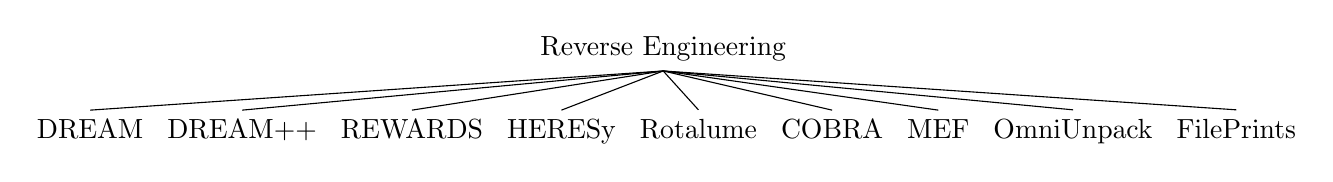
\begin{tikzpicture}
			\Tree
			[.Reverse\ Engineering [.DREAM ][.DREAM++ ][.REWARDS ][.HERESy ][.Rotalume ][.COBRA ][.MEF ][.OmniUnpack ][.FilePrints ]]
			\end{tikzpicture}
			\caption{Malware Reverse Engineering Techniques}\label{Reverse}
		\end{figure}


	\section{Techniques to prevent IT Networks from Malwares}
	\subsection{Distributed Intrusion Detection System}
	With the development and accessibility to new and cheaper technology, there is a proliferation of heterogeneous computer networks which may add difficulty to intrusion detection system. With greater connectivity, the outsiders have more opportunity for accessing vulnerable systems and insiders can avoid detection. Secondly, Network user identification problem where a user can move across systems to defy the current Intrusion detection system's adds another level of attack vector. Problem with using a single point of audit is that multiple host computers can produce large amount of data which needs to be analyzed by a single IDS (Intrusion Detection System) machine and creates an overhead. The attacks that a normal IDS can’t detect includes, an attacker trying to discover insufficiently protected system where the attack activity is lower than the once that can be detected by IDS, i.e. Using the technique of diffusion. Secondly, an attacker can try to access the files using multiple compromised hosts, which can have detected when data from multiple sources is aggregated and correlated. There is always a trade-off between sending limited data from host to IDS versus an attack that could be missed.
	The Distributed Intrusion Detection System architecture~\cite{snapp1991dids}combines distributed monitoring, data reduction and centralized data analysis. A Distributed Intrusion Detection System has following features:
	\begin{itemize}
		\item The host and LAN monitors are used to collect evidence of unauthorized or suspicious activities and DIDS director is responsible for analysis of collaborated data
		\item The architecture is responsible for monitoring bidirectional communications between DIDS director and host machines, which includes notable events and anomaly reports. The director can access more detailed report based on an event and can also update monitoring capabilities on individual hosts.
		\item A large amount of packet filtering is performed at host level to minimize additional network bandwidth.
	\end{itemize}
	There are various components involved in a Distributed Intrusion Detection System. The \textit{DIDS Director}, consists of three components that are logically independent processes and can be hosted in distributed or centralized system. The communication manager, is responsible for moving data between each host, director and LAN monitors. It receives data or make requests with host and LAN monitors. Expert system, receives the data collected by the communication manager from hosts and LAN monitors. It evaluates and reports the security state of individual hosts and the overall network system. User Interface, provides a System Security Officer an interface to watch activities of hosts and network as whole. It can also be used to request specific information about events, host or LAN. The Network-user IDentification (NID), provides a solution to multiple user identity problem, where an attacker can move across hosts to prevent detection in the system. It creates a unique Network User Identification for every new user that enters the system and same NID is used to track activities of the user in the monitored environment. The Host Monitor, watches audit records of transactions on the system that includes file access, system calls, process execution and logins. The host monitor decides whether the transaction needs to be forwarded to the expert system for further evaluation. Critical records are forwarded automatically; others are processed by the local monitors on the hosts. It creates an abstract object called an event to define an activity. Each event is associated with a corresponding action and a domain. A subset of events is forwarded to Expert system for further analysis. The LAN Monitor, observes each packet on its part of the LAN and uses them to construct higher level objects such as connections and service requests using the TCP/IP Protocol or UDP/IP Protocols. It audits host to host connections, network services and traffic volume per connection. It creates profiles of expected network behavior. It also uses data analysis and correlation heuristics to identify possible intrusive behavior of any individual connection. It also helps in creation and use of Network Identifications (NIDs). The Expert System, uses a rule based system where rules are derived from hierarchical \textit{Intrusion Detection Model}. It describes transformation from raw data to higher level abstraction used in describing an attack on a network of computers. The Intrusion Detection Model Process is further divided into six layers:
	\begin{enumerate}
		\item The audit records are received from the host monitors of each individual host operating system and LAN monitors.
		\item The events are created for the audit data which are syntactically and semantically independent of source standard format.
		\item IDM identifies subject from data. A subject defines single identification for a user across several hosts on the network. The subjects are assigned respective Network Identifications (NIDs). After this layer, the entities are defined using subjects and local identification is lost.
		\item At this layer, the subject and event are identified with a context. The set of events are identified as temporal context or spatial context.
		\item This layer evaluates threats to the network and the hosts connected to it. Events are aggregated and combined to define abuses. Abuses are divided into attacks, misuses and suspicious acts. The targets of abuse are identified as system objects or user objects and as being active or passive.
		\item The model produces a numeric value from 1 to 100 which represents overall security state of the network system.
	\end{enumerate}
	Using the Distributed Intrusion Detection System, we can leverage LAN structure to monitor user behavior for attacks against the system and can identify attackers moving across multiple host machines using segregation and aggregation of data from multiple host machines. Also, filtering data at hosts provide optimized learning of the Expert System. This system can be extended to large networks.
	\subsection{SNORT}
	Most of the current Network Intrusion Detection systems (NIDS) for malware analysis face the basic problem that the updates are released at regular intervals of time and malwares are detected or analysed at uneven intervals of time as a result of which systems are vulnerable for phases or intervals. The customers have to wait for vendors to release updates to the vulnerabilities. Secondly, Commercial Network Intrusion Detection Systems are very expensive which makes them inefficient for smaller business networks and devices. With the imminent growth of Internet of Things (IoT) devices there is a need of lighweight and cross platform resources.
	Snort~\cite{roesch1999snort} is a lightweight and cross platform NIDS that can be used for both monitoring network packet data and create an inference based on the traffic to define an attack. The administrator can take define suitable actions, manually or automatically, based upon the alerts.
	A Snort system consists of following components:
	\begin{itemize}
		\item The Packet Decoder
		\item The Detection Engine
		\item The Logging/ Alerting Subsystem
	\end{itemize}
	This further serves many features. Snort is a lightweight and cross platform system allows deployment on any of the nodes, from a large system like mainframe to a small IoT device like raspberry Pi. The small system footprint and easy configurability allows easy implementation of specific security solutions in short time. Rule based logging allows pattern recognition using advanced algorithms allows a variety of attack detection like buffer overflow, SMB probes, CGI attack with creating proper alerts in the respective domain like Server Message Block, Win Popup or an alert file. It decodes the packet from data link layer to the application layer, which allows rules could be implemented on data. This helps in detecting hostile activity including CGI scans, buffer overflows, or unique malware payload using finger print matching.
	Thus considering all the features snort has to offer, we can use it as a Network Intrusion Detection System which is small and flexible and can be used
	
	\subsection{Improving Network Management with Software Defined Networking}
	We can use Software Defined Networking (SDN)~\cite{kim2013improving} to counter the problems of network management and configuration. This is a proactive approach of prevention of malware using vulnerabilities in the network. It works by separating the data plane and the the control plane making switches as forwarders and using a logically centralized program to control the behavior and policies of the entire network. In Software Defined Networks, a central program (controller), defines the behavior of the whole network (control plane) and network devices become simple packet forwarding tools (data plane).
	A software defined networking provides following features:
	\begin{itemize}
		\item Centralized management over the distributed management
		\item Centralized controls allows network configuration changes in a controlled way
	\end{itemize}
	 A software defined network architecture can be implemented using Procera[3], which offers event driven network control framework. A Procera system is developed over a functional reactive programming where policies can be expressed in high level language.We can create a network environment that prevents attack by using data from multiple control domains like time, data usage, privileges for user in the network and flow or network behaviors where network is considered a single identity. 
	 A Software Defined Network like Procera has following components:
	 \begin{itemize}
	 	\item Event Sources, create dynamic events for controller, Intrusion Detection System (IDS) and authentication Systems. The structure of events is defined by corresponding parser in Policy Engine.
		\item The Policy Engine, parses network policy defined by the Policy language. The behavior of policy engine is defined by the policy language and the asynchronous events created by the event sources.
		\item Network Controller, is the central control that translates network policy to actual forwarding rules and manages them over OpenFlow capable switch using openFlow protocol.
	 \end{itemize}
		Thus using this technique, we can accomplish optimized and secured low level configuration of devices in a network. This can also prevent a malware that has infected a single host to infect the whole network as point of breach could be detected by mismatch of policies at the network Controller. Thus, provides a preventive method for malware to move across the network and infect other systems.
	
	\subsection{Malware Detection using Analysis of deviations in Application Network Behavior}
	The intend of this paper~\cite{shabtai2014mobile} is to identify malicious applications on a mobile device, identify add on that could have infected a genuine application or malwares that have self updating capabilities which cannot be detected by standard signature matching approach. This malware detection technique has following features:
	\begin{itemize}
		\item It uses the patterns in network traffic which are specific to each application.
		\item It can rate the levels of deviation from normal behaviors.
		\item It can detect malware that change their signatures with regular updates, dynamic loading of compiled android code, dynamic loading of shared object file or dynamic loading of a shared file.
		\item It can run on mobile devices without much overhead on performance.
	\end{itemize}
	This technique has a stepwise approach and functions according to these components. Graphical User Interface, provides an interface for communication with the user and allow the application configuration based on user requirement. Alert Manager, to manage alerts with user. Feature Extraction, tracks the in/ out data from the device on each type of network in different application states with a track on application’s activity or modification time. Feature Aggregator, provides concise data based upon data extracted in the previous step. It uses average, standard deviation, min-max of sent or received of transmitted data. Local learner, uses semi supervised anomaly detection technique. It employs cross feature analysis to find correlation between data and assumes that a strong correlation means a normal behavior of the application. Anomaly Detection, classifies network behavior based on the correlation data created in the previous step. If there is high correlation in between data of different features, it can be tagged as a normal behavior. If there is low correlation between data, it can be tagged as an anomalous behavior.
	Using this technique, a malware can be detected by monitoring the network traffic in a mobile device. Even if the malware was not detected previously and locked using its specific signatures, we will still be able to detect it using its network behavior. This solution can be used to protect thin clients from malware attacks.
	
	\subsection{Network Intrusion Detection and Countermeasure Selection in Virtual Network Systems}
	This technique provides analysis about using network level activities to find unique vectors that can be used to back-up insights provided by system level activities. These unique behaviors can be further used to collect and classify information and eventually mitigate malicious software~\cite{chung2013nice}.
	They have created an in-depth analysis of malware network behavior using the Sandnet system over a period of 12 months. Sandnet counters two limitations, short analysis period and lack of detailed network behavior analysis which provides an overview of network protocols used by the malware, namely DNS and HTTP. 
	The NICE framework provides following features:
	\begin{itemize}
		\item A distributed network intrusion detection and prevention method in virtual environment using the network traffic of the cloud.
		\item It provides a solution for contingency in case of attack or malware is detected to have compromised the systems in the cloud. It can improve the attack detection probability by aggregating data of network as a single identity.
		\item It uses the attack graph model, where each node represents a system in the cloud and connections are represented using edges. Threats are detected by correlating data from events or activities over the cloud in an attack workflow and hence, suggest effective counter measures based on that.
		\item It adds lesser overhead as compared to other proxy based solutions.
		\item It considers attack as an insider or an external breach of information. Hence, provides more secure solution.
		\item It uses a VM protection model, to maintain a state diagram of the current states of virtual machines in the cloud. Each machine in the network is assigned a stable, vulnerable, exploited or a zombie state.
	\end{itemize}
	This framework works on the following components. Network Intrusion Detection System agent, is used to sniff traffic across the bridges in a cloud server. VM profiler, creates an attack graph for the infrastructure, populating specific alert in NICE agent and records the traffic pattern in a network controller. Attack Analyzer, provides attack correlation and analysis operation based upon the attack graph and logs the threat information to the network controller based on analysis. Network Controller, implements the counter measure based upon the data from attack analyzer by virtual network reconfiguration using the OpenFlow protocol.
	The technique provides a Sandnet system for data collection using network analysis which can be used for prolonged period of time. A network activities overview of 100,000 malwares and augment the data with previous efforts. And an in-depth analysis of DNS and HTTP traffic to define protocol specific usage behaviors of malware. 
	As a conclusion we make a tree structure of various techniques employed by malware detection strategies in IT networks. This can be described as Figure~\ref{Networks}\\
	\begin{figure}[h]
		\centering
			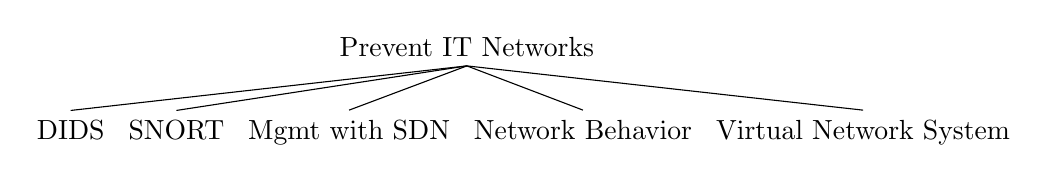
\begin{tikzpicture}
		\Tree
		[.Prevent\ IT\ Networks [.DIDS ] [.SNORT ] [.Mgmt\ with\ SDN ][.Network\ Behavior ][.Virtual\ Network\ System ]]
		\end{tikzpicture}
		\caption{Detect Malwares in IT networks}\label{Networks}
	\end{figure}
	
	\section{Techniques to perform Malware Analysis for Malwares on Android Devices}
	Google’s Android System is a comprehensive software framework targeted towards smart mobile devices which includes an operating system based on the popular Linux OS, middleware and a set of key applications. It is an open-source and community based framework which provides APIs to most of its software and hardware components. Specifically, it allows third-party developers to develop their own applications. The applications are written in the Java programming language based on the APIs provided by the Android Software Development Kit (SDK) and compiled to Dalvik bytecode, but developers can also develop and modify kernel-based functionalities as well.
	Due to the ubiquity and prevalence of smart mobile phones, of which Android has a tremendous 88\% market share, it has become a frequent target of malicious attacks through malware, spyware, viruses, trojans, etc, under the guise of legitimate applications. This necessitates research in providing frameworks and systems to detect and protect our smartphones.
	Various methods have been devised in this regard. Two commonly seen approaches are static and dynamic analysis of malware. The former examines the malware without running the application, using methods of source code and binary analysis for hints of malicious intent, whereas the latter executes the malware in a controlled and monitored environment to observe its behavior. In this part of our project, we will survey a few papers which have proposed techniques and systems to achieve the aforementioned and discuss their methods. 
	
	\subsection{Andromaly}
	Andromaly~\cite{shabtai2012andromaly} is a framework for detecting malware on Android mobile devices which uses a Host-based Malware Detection system that continuously monitors various features and events obtained from the device and applies Machine Learning techniques to detect anomalies by classifying the data as either normal or abnormal. Due to the ‘system-centric’ security model of Android, in which applications statically identify the permissions that govern the rights to their data, the application/developer has a limited ability after installation to dictate to whom those rights are given to or how they are used at a later time. To overcome this limitation, the authors have proposed a lightweight malware-detection system to assist users in detecting suspicious activities on their phones. 
	The detection process consists of real-time and continuous monitoring, collection, preprocessing and analysis of various system metrics such as CPU consumption, number of sent packets through WiFi, number of running processes, battery level, and system usage parameters (e.g., keyboard presses, application startup, etc). After the collection and preprocessing stages, the metrics are sent for analysis to detection units termed ‘processors’ each of which employs its own methods for detecting malicious behavior and outputs a ‘threat assessment’. After this, a notification alerting the user is displayed if malicious behavior is found. The GUI portion of the framework then provides the user with automatic or manual actions which can be chosen to mitigate the threat.
	The main components of the system are discussed in more detail below:
	\begin{itemize}
		\item Feature Extractors – These communicate with various components of the Android framework, including the kernel and Application framework layer in order to collect feature metrics.
		\item Feature Manager -  This component triggers the feature extractors and requests new feature measurements every predefined time interval. It may also apply some preprocessing on the raw features which are collected by the extractors. 
		\item Processor – this component is an analysis and detection unit. It should be provided as a pluggable and modular external component which can be seamlessly installed and uninstalled. Its duty is to receive the feature vectors from the Main service, analyze them and output threat assessments to the Threat Weighting Unit. The processors can be rule based, knowledge based, or they can be classifiers/anomaly detectors which utilize Machine Learning methods.
		\item Threat Weighting Unit – this component obtains the results of analysis by the processors and applies a composite algorithm in order to derive a final singular decision regarding the Android device’s infection level. 
		\item Alert Manager – this component receives the final ranking produced by the Threat Weighting Unit and subsequently applies a smoothing function in order to provide a more persistent alert and avoid instantaneous false alarms. Examples of smoothing functions are : moving average and leaky bucket.
		\item Main Service – this component is undoubtedly the most important component. It synchronizes features collection, malware detection, and the alert process and manages the flow of the whole system by requesting new samples of features and sending newly sampled metrics to the processors.
		\item Graphical User Interface (GUI) – this component provides the user with the means to configure the entire system’s parameters, visual alerting, and visual exploration of collected data.
	\end{itemize}
		The proposed framework employs Machine Learning classification methods in the ‘Processors’ component of the system. Under this approach, the malware detector/classifier continuously monitors various features and events obtained from the system and decides whether the observation samples are normal or abnormal. The classifiers used in the paper for experimenting are : k-Means, Logistic Regression, Histograms, Decision Tree, Bayesian Networks, and Naive Bayes. The evaluations of learned classifiers is split into two steps: training and testing, making the method a supervised learning  form of Machine Learning. During the training phase, a set of both benign and malicious features vectors are provided to the system with their correct labels and the classifier is trained on them. During the testing phase, a different collection (testing set) of feature vectors is evaluated by the classifier and  attempts to differentiate between the benign and malicious vectors.
		Another aspect to consider are the problems of over fitting, reduced generality, increased model complexity and run time which occur due to improper selection of the extracted features. This occurs when there are too many features which are redundant or irrelevant. Because of this, proper feature selection algorithms must be used to obtain high levels of accuracy. This paper uses the filter approach to feature selection due to its fast execution time and generalization ability.
		In conclusion, Andromaly is a good approach to tackling the issues of Android malware and the use of Machine Learning algorithms is definitely a viable approach. Feature Extractors were found to be in the critical execution loop and must be optimized aggressively. Furthermore, the detection of anomalies could be even more effective with the use of a smaller number of features and simpler detection algorithms which ensure stringent resource constraints.

	\subsection{AppsPlayground}
	AppsPlayground~\cite{rastogi2013appsplayground} is a framework that automates the analysis of smartphone applications, specifically targeted towards the Android system. It comprises of multiples components each of which employ different detection and automatic exploration techniques. AppsPlayground is meant to analyze applications for both malware and grayware. Grayware refers to applications which are not malicious but can be annoying, for example by leaking private information for a legitimate purpose without the users awareness. AppsPlayground offers a modular solution to these issues by using a multitude of detection techniques: taint-tracing, sensitive API monitoring, and kernel level system call monitoring.	
	We now describe the overall architecture of AppsPlayground. The general framework is built as a virtual machine environment by re-purposing the Android emulator (Qemu) for a dynamic analysis environment. The virtualized environment is essential for providing scalability which is generally not feasible while using real devices. Some of the challenges in designing such a system are: modeling the GUI, devising an efficient exploration strategy (due to the large number of unique program states which an application will generally contain), and context determination.
	AppsPlayground employs various detection techniques:
	\begin{itemize}
		\item Taint Tracing – Playground uses this technique to track privacy sensitive information leakage. It uses a slightly modified version of TaintDroid (an opensource, high performance taint tracing system for Android), which works for Dalvik bytecode only.
		\item Sensitive API monitoring – playground monitors a few system APIs for detecting possibly malicious functionality, for example, the SMS API, which happens to be one of the most exploited APIs for Android. Malicious applications can use this API to send messages to premium rate numbers without the user’s awareness. Playground can record the destination and content of the SMS messages sent by an app, thereby protecting the device by allowing the user to monitor any malicious activity. Similarly, Playground monitors the Java Reflection API and dynamic bytecode loading.
		\item Kernel Level monitoring – this technique is used by Playground to identify known root-exploits. The method it uses is based on vulnerability conditions and is thus immune to code polymorphism. Some examples of root-exploits already found on Android are: Rageagainstthecage/Zimperlich, Exploid, and Gingerbreak.
	\end{itemize}
	The automatic exploration techniques which AppsPlayground uses are: event triggering and intelligent execution. Many API elements in android are event based, which means that applications may register some code to be triggered only when a certain event occurs. Many malicious applications have been found to register for specific events. AppsPlayground will automatically check that this will not happen. AppsPlayground also intelligently drives the user interface of a smartphone application by dynamically defining and exploring models created from window and widget features. It extracts features from displayed user interfaces to iteratively define a model that approximates the application’s logic. It then creates associations between the current features and those extracted earlier using a method known as widget tracking. Search optimizations are also employed to speed up the process by reducing the search space. Playground also uses sequencing policies to determine the next GUI action. Overall, the implementation of AppsPlayground consists of 3000 lines of Java code.
	AppsPlayground was intensively tested in all sorts of areas, including in detecting information leaks and known Android malware such as FakePlayer, DroidDream, and DroidKungFu and was very effective in all of them.
	
	\subsection{DroidScope}
	DroidScope~\cite{yan2012droidscope} is an Android analysis platform which runs on a virtual Android environment. It is a dynamic binary instrumentation tool which can be modified with plugins as the user intends, with the purpose of analyzing various types of malware and other malicious applications. There are two main reasons for choosing virtualization-based analysis. Since the analysis runs beneath the entire virtual machine, it is able to analyze even the most privileged attacks in the kernel. Also, since the analysis is performed externally, its very difficult for an attack within the virtual environment to disrupt the analysis. It is not without a downside, however, and that is the loss of semantic contextual information when the analysis component is moved out of the box. Also, to enable the virtualization based analysis approach, there needs to be a mechanism to construct semantic knowledge at two levels: at the OS level, and the Java level. With these points in mind, the authors of this paper have designed and implemented DroidScope, which is built on top of QEMU (an Android emulator) which is able to reconstruct both aforementioned semantic views from the outside. DroidScope also provides a set of APIs to help analysts implement custom analysis plugins for whatever purpose they wish.
	The entire Android system, including the malware, runs on top of an emulator, and analysis is performed from the outside. To ensure the best compatibility with virtual Android devices, the authors extended the QEMU by reconstructing the OS level and Java level views simultaneously, implementing dynamic taint analysis, and providing an analysis interface so that future users can build their own custom tools. Several other analysis tools were also developed, such as the API tracer, the native instruction tracer, Dalvik instruction tracer and the taint tracker.
	As mentioned, DroidScope provides a set of APIS to facilitate custom analysis tool development. This is part of an event based interface useful for instrumentation. The APIs provide instrumentation on separate levels: native, OS and Dalvik, so as to mirror the context levels of an actual Android device, and each provides the ability to register callbacks for different events and one can also query or set different kinds of controls. To demonstrate the capability of DroidScope and the types of plugins future users can create themselves, the authors have written 4 of their own analysis plugins: an API tracer, a Native instruction tracer, a Dalvik instruction tracer and a Taint tracker.
	
	\subsection{MamaDroid}
	This technique presents a novel malware detection system for Android, named MamaDroid, that relies on the sequence of abstracted API calls performed by an app rather than their use of frequency, and aims to capture the behavioral model of the app. A key issue that is addressed in this approach is providing resilience to API changes (which often happens) by abstracting specific API calls to either its package name of family name.
	After abstracting the calls, MamaDroid analyzes the sequence of API calls performed by an application, attempting to model its behavior. This is due to the assumption that malware may use the same calls as an ordinary app, but in a different order and for different operations. MamaDroid then  builds a statistical model representing the transitions between the API calls and model these as Markov chains which can then further be used to extract features and perform classification. Another thing to note, is that given the two separate types of abstraction (package or family), both need separate modes of operation. The authors test both extensively and conclude that the abstraction to family is more lightweight, whereas the abstraction to package is more fine-grained.
	The operation of MamaDroid goes through four phases:
	\begin{enumerate}
		\item Extracting the call graph from each app by using static analysis
		\item Obtaining the sequences of API calls using all unique nodes in the call graph and associating each node to all of its children nodes
		\item At this stage, it abstracts the API calls to either package or family and then building on these sequences, it constructs a Markov chain model
		\item Classifies the app as either benign or malware using a machine learning classifier with the transition probabilities used as the feature vector. 
	\end{enumerate}
	For performing classification using Machine Learning, a number of different algorithms were used: Random Forests, 1-Nearest-Neighbor, 3-Nearest-Neighbor, and Support Vector Machines. After extensive testing and experimenting, the results are conclusive that modeling the sequence of API calls as as Markov chain is a successful method of capturing the behavioral model of that application. This fact allowed MamaDroid to obtain a very high accuracy of classification and it promises to retain that level of accuracy over the years, due to the abstraction of specific API calls.
	
	\subsection{Glassbox}
	Glassbox~\cite{irolla2016glassbox} is a functional prototype for the dynamic analysis of malware applications. It executes applications on real devices in a monitored and controlled environment. It is a fully automated system that installs, tests and extracts features from the application for further analysis. The environment is controlled in a way that Glassbox neither users from malware nor becomes an infection vector through the control of web requests, calls and SMS/MMS. The features extracted are Java calls, system calls and both encrypted and unencrypted web requests. In this paper, we present
	the architecture of the platform and we compare it with existing Android dynamic analysis platforms.
	Finally they evaluate the potential of this technique by triggering apps functionalities by comparing the average coverage of basic functionalities on the Auto Coverage database. Some of the features used in this Glassbox system are,
	\begin{itemize}
		\item System calls
		\item Java Calls
		\item Automated testing strategies
	\end{itemize}
	As a conclusion we make a tree structure of various techniques employed by detection of Android malwares. This can be described as Figure~\ref{Android}\\
	\begin{figure}[h]
		\centering
		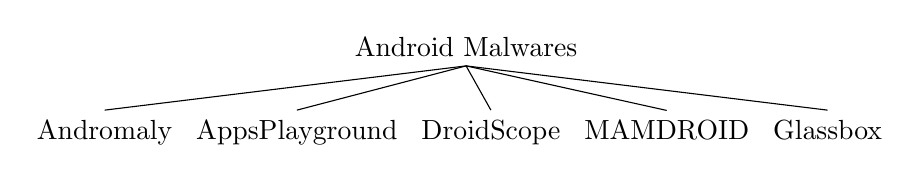
\begin{tikzpicture}
		\Tree
		[.Android\ Malwares [.Andromaly ] [.AppsPlayground ] [.DroidScope ][.MAMDROID ] [.Glassbox ]]
		\end{tikzpicture}
		\caption{Techniques to detect Android Malwares}\label{Android}
	\end{figure}
	

	\section{Techniques for Proactive Defense against Malwares}
	
	Traditional behavioral analysis tends to be a step behind the attackers. To defend against cyber attacks, enterprises have set up response teams but they are usually not effective enough. Sometimes attackers use APT (Advanced Persistent Threat) that is, gaining information on the security measures of the attacked area and elsewhere~\cite{cyberthreatanalysis} by repeated target attacks. As a result, researchers focus on handling APT proactively. Malwares use hooks to register their program into the location~\cite{hookscout}. Rootkits, Network sniffers and other harmful programs use hooks to start their invasion. So, logically, the researchers decided to create a binary-centric hook detection policy which would proactively take care of malware itself. An ideal way to protect from malware attacks is using machine learning and soft computing which is done by Raman Singh and his team of researchers~\cite{softcomputingproactive}. Techniques such as Artificial Neural Networks, Artificial Immune System (AIS) and Fuzzy Set among others were used to combat malware and viruses.  Finally, this report also looked at Muneesh Sharma and Tajinder Kaur’s research on Network Intrusion Detection using Proactive Mechanism~\cite{nidsproactive}. Signature-based defense techniques such as Firewall are less effective when it comes to proactively defending against Malware primarily because they rely on predefined signature sets and are unprepared against newer malwares. So it is still reactive as opposed to proactive. This research makes use of Honeypots to proactively defend against malware. Jianguo Ding~\cite{behaviorbasedproactive} discussed about analyzing malware behavior to proactively defend against unknown malicious codes. \\
	
	\subsection{Cyber Threat Analysis}
	
	Cyber Attacks have become very sophisticated in recent years. Targeted Areas and number of incidents have both increased in alarming quantities. As a result, companies have been forced to adapt an approach where they have to assume that attacks will happen. Sandboxing is one such technique which is used which involves examining files in an isolated environment to check for suspicious behavior. Companies have set up Security Response teams but even they are not enough since damage can happen from leakage of information. The reason for this is APT (Advanced Persistent Threat) which is a repeated targeted attack based on information on security measures. As a result, researchers have begun analyzing APT attacks to develop countermeasures. 
	
	The attack via APT can be described in phases:
	\begin{itemize}
		\item First phase is to prepare for attack by using emails with malware to breach security of the targeted organization.
		\item Second phase is to infiltrate PCs with malware.
		\item Third phase is to construct infrastructure by using backdoor and monitoring networks to collect information on the security system and send this info to intruder’s server.
		\item Next phase is to breach and explore servers to get additional information.
		\item Final phase is to steal valuable information.
	\end{itemize}
	An APT Attack is made with a clear objective. According to the researchers, analyzing these attacks can reveal certain patterns about the attackers. These include features of attack infrastructure, tools (malware), techniques and objective. Such information is called “cyber threat intelligence”. The techniques described in this paper are cyber threat analysis techniques and associated cyber threat intelligence. Some of the techniques used are as follows:
	\begin{itemize}
		\item \textbf{Attack Channel Analysis:} Attack Channel is the technique used by an attacker to infect a terminal inside the targeted organization with malware to enable remote operations. This is usually done by sending targeted emails to a terminal in the organization. This email is analyzed to find information such as email source address, Message Subject, Hostname among other things.
		\item \textbf{Malware Analysis:}This has a three step procedure as follows:
		\begin{enumerate}
			\item Surface Analysis - Analyze the file type, file name, characters in file, etc.
			\item Dynamic Analysis - Running the malware and analyzing its behavior to determine file operation, processes, etc.
			\item Static Analysis - This involves reverse engineering the malware.
		\end{enumerate}
		\item \textbf{C2 Analysis:}  This technique analyzes the C2 server to derive information such as information about IP Address, Location, and Domain Names.
	\end{itemize}
	These techniques have led to the standardization of Cyber Threat Intelligence by releasing specifications such as CybOX, STIX and TAXII. Fujitsu’s have come up with a Proactive Defense Model that uses Cyber Threat Intelligence. There are 6 constituent elements of the model and they are as follows:
	\begin{itemize}
		\item SIEM (Security Information and Event Management) - Consolidates events from a variety of sensors and logs from diverse information systems and assesses whether incident has occurred on the basis of a specific pattern or cyber intelligence.
		\item Incident Management - Manages priority and state of incidents and tasks that need to be executed as tickets.
		\item Artifact storage - Saves artifacts of incidents for use in cyber threat analysis.
		\item Automated Engine - Performs analysis, response and storage of cyber threat intelligence.
		\item Cyber threat intelligence Storage environment - Supports CybOX, STIX and TAXII standards.
		\item Cyber threat Analysis Environment - Analyzes threats to extract new cyber threat intelligence for proactive defense.
	\end{itemize}
	As a future work, the researchers plan to make this model more accurate by trying to extract more cyber threat intelligence. Just using this model is insufficient and collaborating with global vendors and communities is essential.
	
	\subsection{HookScout}
	
	Malware registers its own function (hook) in the target location. Later, the data is registered into EIP and execution is redirected to.malware’s own function. The existing hook detection tools have defeated the older techniques but there are several newer ones evolving. What makes function pointer hooking advantageous for the hackers are the following reasons:
	\begin{itemize}
		\item Attack Space is vast with almost 20000 pointers in Windows Kernel.
		\item It is hard to locate and validate with approximately 7000 in dynamically allocated memory regions. Many of them are in polymorphic data structures which are found in Windows Kernel.
	\end{itemize}
	The goal of this technique is as follows: 
	\begin{enumerate}
		\item To automatically generate a hook detection policy taking advantage of the binary distribution of the OS Kernel.
		\item Locate Function Pointers - To deal with polymorphic data structures.
		\item Validate Function Pointers - Only 3\% ever change in their lifetime. So, a simple policy would be to check if constant pointers ever change.
	\end{enumerate}
	HookScout System has the following parts:
	\begin{itemize}
		\item Monitor Engine - The goal is to determine the concrete memory layout. It also determines primitive types for each memory word for each static/dynamic object. The monitor engine also tracks function pointers. It also does the following work:
		\begin{enumerate}
			\item Running the guest OS within TEMU (Tera-emulator) which is a whole-system binary analysis platform within QEMU (Quick emulator).
			\item For dynamic objects, it performs hook memory allocation/deallocation routines.
			\item For static objects, it executes the hook module loading routine.
		\end{enumerate}
		\item Inference Engine - It infers the abstract memory layout for which it uses context-sensitive abstraction. Object creation context is the execution context where an object is created (e.g. Malloc creator). Objects created under the same context have the same type. The solution is to merge the concrete layouts with the same context into an abstract layout.
		\item Detection Engine - Detection Engine enforces the hook detection policy on user’s machine. 
	\end{itemize}
	To evaluate the performance of HookScout, various aspects were evaluated such as Attack Space, Analysis Subsystem and Detection Subsystem. No false alarms were raised during the testing period. Following limitations were uncovered after the experimental evaluation:
	\begin{itemize}
		\item Coverage - 5 \% of the kernel is not covered which could be exploited by the attackers.
		\item Detection Interval - Deciding the detection interval is tough. 5 seconds or even a second might be too late when it comes to detecting attacks.
		\item Uncommon Proprietary Device Drivers - HookScout utilizes QEMU (Quick Emulator) and since other proprietary drivers are never installed, they are not analyzed.
		\item There are limited test cases for the Dynamic Analysis.
		\item Kernel Module can be subverted or misled. Hypervisor is preferred for this reason.
	\end{itemize}
	Function pointer hooking is a new trend and hard to detect but the researchers have developed HookScout which is proactive, binary-centric and context-sensitive.
	
	\subsection{Threat Intelligence}
	In order to proactively detect and defend malicious software, only analyzing the malware itself may bring us unilateral information and provides incomplete solutions. We need to consider it from another aspect, which is the intelligence. By collecting and analyzing particular intelligence, we will generate new unbelievable useful information that can let us have a big picture of the malware, and obtain new insights of the malicious behaviors, so that we can understand which malware families are popular, how are the most vulnerable targets, and actually come up with proactive detection and dependence approaches.
	Towards Automated Threat Intelligence Fusion~\cite{moditowards}, which was published in 2016 Collaboration and Internet Computing (CIC), to study the threat intelligence analysis. The other paper I read is “Needles in a Haystack: Mining Information from Public Dynamic Analysis Sandboxes for Malware Intelligence”, which was published in USENIX Security 2015. As there are few research papers are about malware and threat intelligence, I decide to read some white papers from particular organizations, such as SONICWALL, CISCO and CYBER4SIGHT.
	In ~\cite{moditowards}, authors propose an Automated Threat Intelligence fusion framework (ATIS) to take all sorts of threat intelligence into account and discover new useful intelligence by connecting the dots of apparently isolated cyber events. 
	Currently, threat analysis and intelligence discovery are still performed piecemeal in an ad-hoc manner. When people analyze the malware, or social network, they just focus on studying the individual aspect, which will produce unilateral intelligence and affect the proactive detection and prevention. In contract, we can figure out a way to integrate all intelligence from different sources, then by analyzing the new knowledge base, it is highly likely to find out useful information that can help predict and against the malware or other kinds of threats. ATIS is well-designed with five planes, which are collection plane, analysis plane, control plane, data plane and app plane. In the collection plane, they design different crawlers to collect data from different sources, such as underground forums, some well-known security service provider official website, malware sample dataset and etc. In the analysis plane, there are several modules are running for analyzing particular type of data source. A logically centralized controller is used for automatic data collection and intelligence discovery by orchestrating the collections and analysis modules. Data plane is used to store discovered intelligence in a global knowledge base. Users can define their own business logic and develop corresponding applications that run in the app plane to perform threat intelligence analysis.
	This paper shows us its effectiveness by two well developed applications, query and social intelligence analysis. Query application is used to show all relevant user-defined type of intelligence within particular hops. Through this application, for example, we can see how a user in the underground forum relates to a malware and the correlation between different cyber-related factors. Social intelligence analysis was performed by an social application. This one only takes advantage of the social-related intelligence in the global knowledge base.
	Through these two examples, analyzing the integrated intelligence can bring more insights that are never noticed before to us and provide use new ideas of proactive detection and prevention.

	\subsection{Mining Information from Public Dynamic Analysis}
	Authors propose a novel approach to identify malware development automatically from the samples submitted to a malware analysis sandbox. In another words, they try to detect if malware makers submit their samples during the malware development phase and get more insights about the dynamics of malware development, which may be used in an early detection and prevention system. 	
	The authors do the study based on two facts:
	\begin{itemize}
		\item It is common that antivirus companies or public malware analysis sandboxes collect the malware samples long before the attacks are disclosed
		\item The criminals are racing with researchers. They need to understand what systems or approaches the researchers are using and then further develop their software to avoid being detected
	\end{itemize}
	Therefore, analyzing all available samples collected by antivirus companies and public sandboxes can provide the intelligence of the malware development. This methodology proposed by this paper adopts dynamic and static malware analysis, as well as machine learning approaches. 
	The approach can be divided into five steps. Firstly, they filter out the samples that are not relevant to this research. Samples that are not disclosed after submitting to the public sandboxes or not submitted manually will be discarded. They will also remove not executable or duplicated files.  Secondly, they cluster the remaining samples based on their binary similarity. After that, Samples in each cluster are then compared using a more fine-grained static analysis technique. Then based on the static characteristics and results from dynamic analysis, they collect six sets of features. Finally, they apply these features to classifiers to do prediction. Results shows that by combining dynamic and static analysis with features with features based on the file submission, it is possible to achieve a high accuracy in automatically identifying cases of malware developments. There are thousands malware development identified and some of them have been later observed on thousands of infected machines around the world. Through the analysis of malware developments, it shows how the authors modify their programs to test their functionalities or to evade detections from known sandboxes. 
	
	\subsection{SONICWALL}
	As there are few research papers talking about intelligence, we also take insight into several white papers to understand the latest malware status around the world and which kind of malware is becoming popular.
	This white paper, firstly reviews malware attacking situation in the overall 2016 and then introduces malware types that deserve our more attentions. According to this report, we have victories against malware in 2016 to some extent. SonicWall only collect 60 million unique malware samples, but the volume is up 64 million in 2015. Total attack attempts dropped for the first time in years, to 7.87 billion from 8.19 billion in 2015. The most exciting part is point-of-sale system attacks has 88 percent decrease in POS malware variants since 2015, because of chip adoption. However, the ransomware threat increase dramatically and becomes one of the most popular malware. There are only 4 million ransomware attacks in 2015, but the number grows to 638 million in 2016. The rise of ransomware-as-aa-service ( RaaS) makes it easier for cyber criminals to deploy ransomware. Additionally, Internet of Things devices are compromising on a massive scale due to poorly designed security features, opening the door for distributed denial-of-service attacks.
	Latest white papers contents confirm the information provided by the SONICWALL report. At least more than half of latest released white papers involve ransomware intelligence, and many of them make individual report only about ransomware.  In their reports, they do not introduce current ransomware status, but also provide proactive prevention advices. CISCO has a report, Ransomware: Everything You Need to Know. This report introduce ransomware briefly, and suggest users what they can do prevent ransomware before an attack, during an attack and after an attack. One thing need to attention from this report is that according to their intelligence, the integrity of decrypted files is a big concern. SONICWALL also writes a report, called 8 ways to protect your network against ransomware, to provide protection advices. This report involves from employee education, technique used to protection to daily operations suggestions. It seems there are no every effective way to against ransomware, except backing up necessary files and the network segmentation. One interesting part need to be pointed out is that Android OS users need to pay more attention on their devices, as they are also valuable targets of the criminals.
	According to the article by Michael Heller, doxware is a new type of ransomware, which will research targeted victims and expose their sensitive information online if the victims don’t pay ransoms. Currently, most of other reports suggest that backing up files is the most important approach to against the ransomware. However, this new type of ransomware may destroy this prevention approach. 
	Report by Booz Allen from Cyber4Sight provides ransomware intelligence analysis. They find out a new RaaS platform named “Satan” is being promoted on the Club2crd forum. The malware is free, but the service operators retain 30 percent of the ransoms paid initially. The users can customize several features of the malware, such as how much the victim need to pay. This RaaS makes users access and use the ransomware easily, and potentially impacts our security situation seriously, as until now we don’t have a perfect approach to predict and prevent against this kind of malware. Through the forum analysis, they find out a user called, Cold\_As\_Ice. By analyzing this user, they think Cold\_As\_Ice could be the actor behind it and highly likely he/she is in Brazil. 
	
	\subsection{Soft Computing Techniques}	
	
	Soft computing techniques are widely used in malware detection these days. These techniques have the ability of learning from past incidents and categorize normal and abnormal behavior. Malware includes viruses, worms, trojan horses, spyware and adware. In recent times, network attacks are easy to launch as the tools to perform such attacks are present freely on the internet. To overcome this problem, IDS (Intrusion Detection System) is used against malicious activity. An IDS monitors the system and decides if the activity is sign of an attack or normal activity. Various soft computing and machine learning techniques are employed in IDS to detect various attacks. 
	Some of the techniques are as follows:
	\begin{itemize}
		\item Artificial Immune System (AIS) - AIS helps solve complex computational problems. Using learning, feature extraction, and pattern recognition, it offers rich metaphors for its artificial counterpart.
		\item Fuzzy Set - Fuzzy Logic is a means of modelling the uncertainty of the natural language. The use of fuzzy logic is in two areas - algorithms with learning and adaptive capabilities with the purpose of automatically designing fuzzy rules and to enhance readability of machine learning algorithms such as Support Vector Machines or Hidden Markov Model.
		\item Artificial Neural Networks (ANN) - ANN learns to predict the behavior of various users and daemons in the system. The main advantage of ANN is the tolerance to incomplete information and ability to infer solutions from the data without prior knowledge of regularities in the data.
		\item Decision Tree - It is a powerful tool for classification and prediction. It has three main components - nodes, leaves and arcs.
		\item Support Vector Machines - They are a relatively new supervised machine learning technique. Although the basic technique was conceived for binary classification, several methods for single and multi-class problems have been developed. The usefulness of SVM has been already demonstrated in several fields: like pattern recognition, where it can provide optimal statistical classification by means of properly chosen decision functions.
		\item Other techniques - These include genetic algorithms, Evolutionary Algorithms, Swarm Intelligence.
	\end{itemize}
	Malware Detection using Soft Computing Techniques is primarily classified in three categories:
	\begin{itemize}
		\item Misuse/Signature Detection - Researchers have developed many techniques based on detecting signature of a malware. Some are:
		\begin{enumerate}
			\item Signature Verification with SVM - Buffer Overflow Vulnerabilities are exploited by worms which can be handled with network-based Length-based Signature Generator (LESG).
			\item Signature Tree Generation - Network-based Generation has been proposed as a way to automatically and quickly generate signatures for worms, especially polymorphic worms. PolyTree, an NSG system is composed of two sections - signature tree generator and signature selector.
			\item Logical Expression Testing Criteria - Decision Support has problems in accurately identifying attacks. Recognizing that signatures in essence provide the specification of an IDS engine, studying the accuracy of an IDS engine becomes a black-box testing problem.
			\item F-Sign - F-Sign is designed for extracting unique signatures from malware files automatically. Malicious executable is analysed using two approaches: disassembly, utilizing IDA-Pro, and the application of a dedicated state machine in order to obtain the set of functions comprising the executable.
			\item Bayesian Network - It is used for intrusion detection. The flexible nature Bayesian network allows it to be used both for misuse-based and anomaly-based detection process.
			\item Semantic aware Signature Generation - String extraction and matching techniques have been widely used in generating signatures for worm detection, but how to generate effective worm signatures in an adversarial environment still remains a challenging problem. Semantics Aware Statistical (SAS) algorithm have been proposed for automatic signature generation.
		\end{enumerate}
		\item Anomaly Detection - Anomaly Intrusion Detection (IDs) strategy considers abnormal behavior is rare and tries to model normal rather than anomalous behavior. Researchers do a lot of work in anomaly detection. Specifically, they use machine-learning algorithm to classify fixed-length patterns generated via sliding window technique to infer the classification of variable length patterns from the aggregation of the machine learning based classification results. Some other techniques proposed by researchers are Feature-Aided Tracking with Hidden Markov Models. Histogram-Based Traffic Anomaly Detection. Anomaly Detection through a Bayesian Support Vector Machine.
		\item Hybrid Detection - Signature based detection system can only detect attacks which are known to system and signatures are defined. Anomaly based detection has higher False-Positive rate. These techniques can be combined to give better results. This combined technique is known as Hybrid detection scheme. A hybrid model is used not only to correlate alerts as accurately and efficiently as possible but also to be able to boost the model in the course of time.
	\end{itemize}
The network data is very large, heterogeneous, highly varying and imbalanced. Real time anomaly detection approaches with high accuracy and low false positive rate are required.
	
	\subsection{A Study of Network Intrusion Detection Based on Proactive Mechanism}
	In this paper, the researchers presented the tools and techniques used to protect the networks and its associated resources and requirements for the proactive network intrusion detection mechanism which should be placed in line with the current intrusion detection system to protect the entire network. Though the general impression is the growing cyber security awareness among the masses, but the advanced hacker techniques and sophistication seems to counter the defensive mechanisms easily and fool the users. The malwares propagating in network have become the biggest threat to the increasing internet. \\ \\
	Countermeasures like firewalls or anti-anything (antivirus, anti-spam, anti-spyware, etc.) are all reactive security tools. They are necessary countermeasures and a part of a comprehensive security system, but you must also take action, be proactive, to ensure the highest level of network security. There is a need to put the place a security mechanism to analyse malicious activity without having rely on the traditional signature based tools. To strengthen these signatures based tools and to manage these tools, there is a need to react proactively so that the analysis of the malicious codes can be performed and signatures for the security can be performed. This research will explain the use of proactive security defence mechanism based on different tools and techniques which help in the creation of a tested that would help in testing and identifying the weakness of a network. There are various types of malwares such as Virus, Worms, Trojans, Spyware, Adware and Rootkits. Most recent operating systems come with built in and “enabled by default” firewall package. Starting with Windows XP service pack 2 and since, firewall has been enabled by default on all Microsoft operating systems. Antivirus software is the basic security tool installed in end user computer. They mostly rely on signature based detection where executable files are matched against a signature database of known viruses. New versions have run-time scanning feature that scans the file in real time and avoids execution, if a threat is detected. Signature based detection however results in the antivirus engine failing to detect variants of known viruses, therefore a constant update of antivirus signature database is essential to provide basic protection.\\ \\
	One promising approach to improve network defense is the use of honey pots, a closely monitored computing resource that we want to have probed, attacked or compromised. More precisely, a honeypot is "an information system resource whose value lies in monitoring unauthorized or illicit use of that resource" Honey pots can run any operating system and any number of services. The configured services determine the vectors available to an adversary for compromising or probing the system. Honeypots can be broadly classified into two types - Server and Client Honeypots. Further both of them are classified each into Low interaction and High Interaction Honeypots. Low Interaction Honeypots emulate a variety of host services. In a High Interaction Honeypot, the attacker is given the freedom to interact with a real operating system and their every attempt is logged and accounted for. The second Honeypot category is also classified based on the way they are deployed in a network as follows:
	\begin{itemize}
		\item Production Honeypots - They are placed within an organization’s production network for the purpose of detection. They extend the capabilities of intrusion detection systems.
		\item Research Honeypots - These are deployed by network security researchers – the white hat hackers. They allow complete freedom for the attacker and, in the process; it is possible to learn their tactics.
	\end{itemize}
	The researchers then talk about the way the honeypots are deployed with the design and process flow and conclude by proposing the system of honeypots which is able to detect the malware programs with the help of honeypot as well as by applying the intelligent forensic investigation of the collected network PCAP (Packet Capture) data.
	
	\subsection{Behavior-based Proactive Detection of Unknown Malicious Codes}
	
	Malicious code is defined as any program that is specifically coded to cause an unexpected (and usually) unwanted event on a User’s PC or Server. There are several types of malware such as Adware, Spyware, Virus, Worms, etc. The antivirus technologies that are present currently are Signature-based scanning,	Heuristic analysis, Cyclic redundancy check (CRC) scanner, Vaccination technology, Behavior blockers, Immunizers, Snapshot technology and Sandbox technology.\\ \\
	There has been an increase in the amount of malicious codes along with polymorphism and metamorphism in malicious codes. Researchers have to deal with any reported unknown malicious code by manual analysis, and then denote a signature for it and update the virus database. This paper tries to establish an automatic mechanism to assistant classifying and identifying unknown malicious codes. There are two types of behavioral analysis techniques. One is static analysis in which the binary code is disassembled and the functions of the program are analyzed without executing it. The second one is dynamic analysis in which we analyze the code during runtime. Malicious behavior can be categorized as File-related behavior, Process-related behavior, Window-related behavior, Network-related behavior, Register-related behavior and Windows service behavior.\\ \\
	The paper then describes the analysis methods particularly, Statistic-based method and MoE (Mixture of Experts) Neural Network Model. Two experiments were conducted where the MoE model showed a better performance although both did not get the detection rate to 100\%. Ultimately, the researchers concluded that a single method cannot get the best result.  The detection rate did not reach 100\% because definition of malicious codes changes with users. As a future research, a larger data set was proposed for the experiment and finding other ways to improve proactive detection.	
	As a conclusion we make a tree structure of various techniques employed by proactive detection of malwares and threat intelligence. This can be described as Figure~\ref{proactive}\\
	\begin{figure}
		\centering
			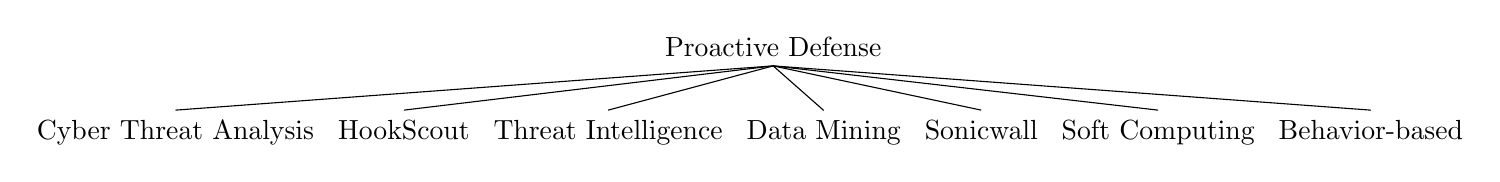
\begin{tikzpicture}
		\Tree
		[.Proactive\ Defense [.Cyber\ Threat\ Analysis ] [.HookScout ] [.Threat\ Intelligence ][.Data\ Mining ] [.Sonicwall ][.Soft\ Computing ][.Behavior-based ] ]
		\end{tikzpicture}
		\caption{Proactive Detection Techniques}\label{proactive}
	\end{figure}
	
	

	\section{Conclusion and Recommendations}
	\subsection{Tree Structure of Tools \& Techniques}
	After studying a part of the extensive literature on Malware Anlaysis techniques, proactive detection and prevention we came to a conclusion to make a tree structure about various techniques and tools we studied. This structure is presented in the diagrams. It gives a precise idea of the whole survey article. When we started of with this project we together came up with this idea and making this as our major result. At the end of each section we present you with this tree structure
	As we can see the root node of this tree is our topic and the children are followed according to our project goals and literature studied on the topic. We provide with these trees as our study on techniques to perform malware analysis and how to proactively prevent and detect them.
	The tree structure in which we present our article can be described as follows:\\
	\begin{figure}[h]
		\centering
			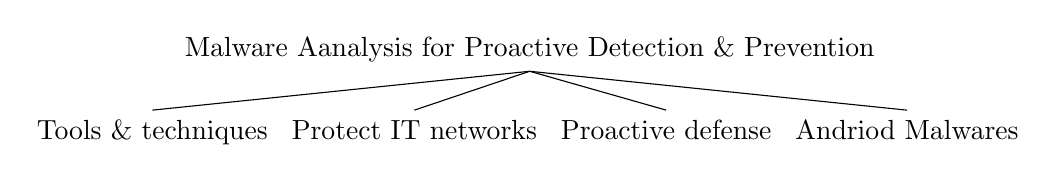
\begin{tikzpicture}
		\Tree
		[.Malware\ Aanalysis\ for\ Proactive\ Detection\ \&\ Prevention [.Tools\ \&\ techniques ] [.Protect\ IT\ networks ] [.Proactive\ defense ][.Andriod\ Malwares ] ]
		\end{tikzpicture}
		\caption{Summary of goals}\label{goals}
	\end{figure}
		
	
	\subsection{Prevent Malwares on the Network itself}
	This section explains you the results we obtained from our survey article about techniques to prevent IT network from Malwares. We observed that detection of malware can also be done on the network level. Various tools can be used to continuously monitor the network traffic to check for malware signatures. These we represent previously in this article at ~\ref{Networks}. 
	These techniques generally employ detection strategies based on the packet flowing into the network. Methods like deep packet inspection are also widely known now-a-days inorder to perform this detection. However, malwares not every time come via web traffic. As examples suggested many a times malwares are deployed through a USB or physically. When this things happen it is difficult to detect malware till it gets executed and generates traffic out of the network. Still, it is important to understand how things can be done on network level to add a layer of  defense against malware.
	
	
	\subsection{Analyze Android Malwares}
	This section explains you the results we obtained from our survey article about techniques to perform Malware Analysis for Malwares on Android Devices. We have seen that there exist many different approaches to malware detection on Android systems. Ubiquitously, dynamic analysis is considered to be far more advantageous than static analysis on this system, particularly due to the ease of code obfuscation. Another trend we can observe is the use of Machine Learning to learn the various models of the types of malware in operation currently. This idea has a lot of potential and I believe with the progress of machine learning techniques and algorithms, malware analysis will continue to become better and better and perhaps malware on Android systems will be vanquished entirely. On this point, one observation I’ve made is that these papers generally use generic and slightly deprecated Machine Learning algorithms (such as Naive Baye’s and SVM classifiers). This is mostly due to the focus of many of these papers on primarily creating a novel framework or system and the fact these authors perhaps aren’t as well versed in current Machine Learning research as current Malware Analysis research. We think this is definitely an area of improvement which could further the prospects of their research and results. With the advent and current popularity of Neural networks and Deep Learning techniques, we would imagine that using these techniques might improve their results if they were used appropriately. 
	We try to represent these techniques in a tree structure as below.\\
		
	
	\subsection{Proactive Defense against Malwares}
	This section explains you the results we obtained from our survey article about techniques for proactive defense against malwares.Through reading the papers and white papers, we studied the malware proactive detection and prevention from two aspects. One is from the analysis of the malicious software itself dynamically and statically. The other one is through threat intelligence to detect and prevent from malware. By reading these papers, we saw most of effective analysis approaches, including intelligence generation, need to involve both of dynamic analysis and static analysis.  Traditional analysis can solve many of threats, but intelligence analysis can give us more insights about the malicious behaviors and events, which can help use design new comprehensive proactive detection and prevention strategies. We try to represent these techniques in a tree structure as below\\
	
	\subsection{Tabular summary of techniques employed by different Tools}
	In the article we talk about various tools which are in the wild to perform static or dynamic analysis of malwares. In this section we summarize all the techniques we studied used by various malware analysis tools. This also allows us to compare these tools when we think about using any tool to perform malware analysis. Considering these techniques implemented we can also think about mixing and matching these techniques to build a more intelligent and improvised tool.
	\begin{table}[h]
		\begin{tabular}{l l l l }
			\hline
			Sr. No & Tool & Technique\\
			\hline
			1 & Ether & Virtual Machine Monitor,API calls Single stepping\\
			\hline
			2 & V2E & Virtual Machine Monitor, Recording and replay\\
			\hline
			3 & SPIDER & KVM Hypervisor, Code Instrumentation and Debugging, Split Code and Data view\\
			\hline
			4 & DRAKVUF & LibVMI, Direct Memory Access, Rekall, Volatility\\
			\hline
			5 & DREAM & Decompiler, Control Flow Graph, Abstract Syntax Tree\\
			\hline
			6 & DREAM++  & Decompiler, Simple flow structures\\
			\hline
			7 & REWARDS & Decompiler, Determine data structures, Type Sinks\\
			\hline
			8 & HERESy & Honeypot, Reverse Engineering, Containers\\
			\hline
			9 & Rotalume & Reverse Engineering, Malware Emulators, Analyzes emulators not malwares\\
			\hline
			10 & COBRA & Fine grained analysis, Localized Execution, Block Coalescing, Stealth\\
			\hline
			11 & MEF & UNIX mail server, Naïve Bayes Classifier, MD5 Hash\\
			\hline
			12 & OmniUnpack  & Monitor System Calls, Memory Access, User space malware detector\\
			\hline
			13 & Andromaly    & Machine Learning, K-means, Logistic Regression, Feature Extractors\\
			\hline
			14 & AppsPlayground   & Grayware detection, Taint tracing, Kernel level monitoring, API monitoring\\
			\hline
			15 & DroidScope  & Dynamic Binary Instrumentation, Dynamic Taint Analysis, Dalvik Instruction Tracer\\
			\hline
			16 & MamaDroid   & Resilient to API changes, Markov Chains, Machine Learning\\
			\hline
		\end{tabular}
	\caption{Summary of Techniques used by various Tools}
	\label{tab:summary}
	\end{table}

	
	\subsection{Recommendations}
	Fight against Malwares is the most required thing in the Security as well as IT world today. After studying the literature over this topic we came to some recommendations by which this fight against malwares can be further improved.
	\begin{enumerate}
		\item Designing automated tools to detect malwares is a task we can be improvised. There are various techniques like static program analysis, constraint solving, symbolic code execution which can be used in order to make these tools. A malware reverse engineer uses tools like IDA pro and gnu debugger to reverse engineer the malware binaries. Automated tool can perform these things and try to gain more information about execution of malware without running it. So, this technique will prevent us from executing the malware in a sand-boxed environment.
		
		\item We can also make improvements in the techniques to detect malware on the network level. Current techniques implement, packet inspection to determine whether any packet has malicious code in it or not. But even these techniques don't allow us to exactly identify whether the code is indeed malicious or no. This generates a lot of false positive and can harm benign traffic flowing in the network. We can use software defined network in order to perform deep packet inspection of every packet flowing in and out of the network. Various concepts like hoenypots can be used to lure the traffic and detect behavior of this malicious code. Once we learn its behavior various blocking constraints can be implements on the original network.
		
		\item Current research is going on the hot topic of threat intelligence. Malware analysis module is the most important part in order to generate intelligence. Researchers and Industry professionals are now stressing on having an Intelligent Security Operations Center which will provide them with live threat reports and keep them updated against current Zero day vulnerabilities. After reading the literature available on this topic we feel that there is a lot of work which can be done in this area. There is a whole different world present in the so called and well known dark web. On this inter-network, which is not cached by public crawlers like Google, Yahoo, people share and upload whole new level of content which is illegal, obscene or malicious. If we want to have a really good threat intelligence feed then we should not neglect this inter-network. So we think that, crawling the dark web will also provide humongous amount of threat intelligence. Many of the BlackHat guys are known to publish zero day exploits on this websites. Hence, if we have live constant feed of these details then our security operations center can be one step ahead in proactively defending against malwares. Threat intelligence can also be gained by analyzing malwares using various Tools we studied in this article. One such technique was used by ~\cite{moditowards}, which is maintaining a datastore of analyzed malware and gaining pieces of intelligence from these analyzed malware as threat feeds.
		
		\item Bring-Your-Own-Device is a new thing today in the corporate world. Employees are allowed to access the company VPN through their mobile device. Due to this, the malware community has got a new direction and motivation to write malwares. This community is now constantly evolving in scripting malwares for Android as well as iOS devices. In this article we studied the literature available on techniques to detect android malwares. In addition to this, research can also look into various techniques to detect iOS malwares. 
	\end{enumerate}

\bibliographystyle{plain}
\bibliography{biblio}
\end{document}

